\documentclass{article}
\usepackage[utf8]{inputenc}
\usepackage{amsfonts, amsmath, amssymb}
\usepackage[english]{babel}
% \usepackage{boisik}
\usepackage{amsthm}
\usepackage[margin=0.5in]{geometry}
\usepackage{MnSymbol,wasysym}

%\usepackage{tgbonum}
%\usepackage{cmbright}
%\usepackage{textcomp}
\usepackage[object=am]{pgfornament}
\usepackage{graphicx}
\usepackage{tikz-cd}

\usepackage{sectsty}

\sectionfont{\fontsize{20}{20}\selectfont}


\subsectionfont{\fontsize{15}{15}\selectfont}


\theoremstyle{definition}
\newtheorem{definition}{$\boxed{\star}$ Definition}
\newcommand{\tit}[1]{\textit{#1}}
\newtheorem{theorem}{$\boxed{\boxed{\circledast}}$ Theorem}

%\newcommand{\nll}[0]{\newline\newline}
\theoremstyle{remark}
\newtheorem*{remark}{Remark}

\theoremstyle{definition}
\newtheorem{corollary}{$ \to $ Corollary}

\theoremstyle{definition}
\newtheorem{proposition}{$\checkmark$ Proposition}

\theoremstyle{definition}
\newtheorem{doubt}{$\boxed{?}$ Doubt}

\theoremstyle{proof}
\newtheorem*{attempt}{Attempt}

\title{Month of Topology \& Abstract Algebra\\
	\large Abstract Algebra - Definitions, Propositions, Theorems \& Proofs}
\author{Animesh Renanse}
\date{\today}
\usepackage{amsthm}

\newcommand{\abs}[1]{\left \vert#1\right \vert}
\newcommand{\inv}[1]{#1^{-1}}
\newcommand{\gen}[1]{\left\langle #1\right\rangle}
\newcommand{\order}[1]{\left\vert #1 \right\vert}
\newcommand{\image}[0]{\text{Im }}
\newcommand{\kernel}[0]{\text{Ker }}
\newcommand{\nsg}[0]{\trianglelefteq}
\newcommand{\isomorph}{\cong}
\newcommand{\End}[1]{\text{\textbf{End}}\left(#1\right)}
\newcommand{\Auto}[1]{\text{\textbf{Aut}}\left(#1\right)}
\newcommand{\Id}[1]{\text{Id}_{#1}}
%\makeatletter
%\newcommand*\bigcdot{\mathpalette\bigcdot@{.5}}

\renewcommand{\qedsymbol}{\ensuremath{\blacksquare}}


\begin{document}
	
	\begin{titlepage}
		{\scshape\LARGE Indian Institute of Technology, Guwahati \par}
		\vspace{1cm}
		{\scshape\Large Pre-Final Year : $ 6^{th} $ Semester\par}
		\vspace{1.5cm}
		{\Huge\bfseries Abstract Algebra\par}
		\vspace{2cm}
		{\Large\itshape Animesh Renanse\par}
		\vfill
%		Instructed by\par
%		Prof.~Tony \textsc{Jacob}
		{\large \itshape Self-Study Notes\par}
		\vfill
		
		% Bottom of the page
		{\large \today\par}
	\end{titlepage}
\tableofcontents
\newpage
	\textbf{Target : }\textit{Reach Field Extensions.}
%	{Commutative Rings}
%	\hrulefill
%	\begin{definition}
%		A \textbf{ring} $R$ is a set of two binary operations $R\times R \to R$: addition $(a,b)\to a+b$ and multiplication $(a,b) \to ab$, such that,
%		\begin{enumerate}
%			\item {$R$ is an \textbf{Abelian Group under addition}, that is,
%				\begin{equation}
%					\begin{split}
%						a+(b+c) &= (a+b) + c\\
%						\exists \;0 \in R\;\;\text{such that}\;\;0+a &= a\\
%						\exists\; a^\prime \in R\;\;\text{such that}\;\; a + (a^\prime) &= 0\\
%						a+b &= b+a
%					\end{split}
%				\end{equation}
%			}
%			\item{\textbf{Associativity} : $a(bc) = (ab)c$ for every $a,b,c \;\in \;R$.}
%			\item{\textbf{Identity} : There is $1 \in R$ with $1a = a = a1$ for every $a\in R$.}
%			\item{\textbf{Distributivity} : $a(b+c) = ab+ ac$ and $(b+c)a = ba+ ca$ for every $a,b,c \in R$. }
%		\end{enumerate}
%	\end{definition}
%	\hrulefill
%	\begin{proposition}
%		Let $R$ be a Ring,
%		\begin{enumerate}
%			\item {$0\cdot a = 0 = a\cdot 0$ for every $a\in R$.}
%			\item{If $1 = 0$, then $R$ consists of the single element $0$. In this case, $R$ is called \textbf{Zero Ring}.}
%			\item{If $-a$ is the additive inverse of $a$, then $(-1)(-a) = a = (-a)(-1)$. In particular, $(-1)(-1) = 1$.}
%			\item{$(-1)a = -a = a(-1)$ for every $a\in R$.}
%			\item{If $n \in \mathbb{N}$ and $n1 = 0$, then $na=0$ for all $a\in R$. Recall that if $a\in R$ and $n\in \mathbb{N}$, then $na = a + a + \dots + a$ (n summands).}
%		\end{enumerate}
%	\end{proposition}
%	\hrulefill
%	\begin{definition}
%		A subset $S$ of a Ring $R$ is called a \textbf{Subring} of $R$ if,
%		\begin{itemize}
%			\item{$1\in S$}
%			\item{If $a,b\in S$, then $a-b \in S$.}
%			\item{$a,b \in S$, then $ab \in S$.}
%		\end{itemize}
%		A \textbf{Proper} subring $S$ is usually denoted as $S\subsetneq R$.
%	\end{definition}
%	\hrulefill
%	\begin{proposition}
%		A subring $S$ of a ring $R$ is itself a ring.
%	\end{proposition}
%	\begin{proof}
%		From $1.$ and $2.$ of the definition of rings, we see that a subring has $+$ and $.$ operations. Furthermore, since $S$ is a subset of $R$, thus it's elements also follows the associativity and distributivity rules.
%	\end{proof}
%	\textbf{Example.} $\mathbb{Z}[\xi_n] = \left\{ a_0 + a_1\xi_n + \dots + a_{n-1}\xi^{n-1}_n \in \mathbb{C}\;:\;\;a_i \in \mathbb{Z} \right\}$ is a \textbf{subring} of $\mathbb{C}$ where $\xi_n = e^{\frac{2\pi i}{n}}$.
%	\hrulefill
%	\begin{definition}
%		A ring $ R $ is called a \textbf{Commutative Ring} if $ ab = ba $ for all $ a,b \in R $. That is, it's also commutative over the ring's multiplication operation.
%	\end{definition}
%		\textbf{Examples.} $ \mathbb{R,Z,Q} $ and $ \mathbb{C} $ are commutative rings.
%	\hrulefill
%	\begin{proposition}
%		\tit{(\textbf{Binomial Theorem})}. Let $ R $ be a Commutative Ring. If $ a,b \in R $, then,
%		\begin{equation}
%			(a+b)^n = \sum_{r=0}^{n} \binom{n}{r} a^r b^{n-r}
%		\end{equation}
%	We have the following immediate result.
%	
%	\textbf{Corollary}. If $ N\in \text{Mat}_n(\mathbb{Z}_p) $, then $ (I+N)^p = I+N^p $.
%	
%	where , if $ k $ is a commutative ring then, $\text{Mat}_n(k)  $ is the set of all $ n\times n $ matrices with entries in $ k $, a ring and $ \mathbb{Z}_p $ is the \textit{integer mod $ p $}, where $ p $ is a prime number.
%	\end{proposition}
%\hrulefill
%\begin{definition}
%	A \textbf{domain} or an \textbf{integral domain} \textit{(a collection of integers in German)} is a commutative ring $ R $ which satisfies the following two extra axioms:
%	\begin{enumerate}
%		\item{$ 1\neq 0 $.}
%		\item{\textbf{Cancellation Law} : For all $ a,b,c\in R $, if $ ca = cb $ and $ c\neq 0 $ then $ a=b $.} 
%	\end{enumerate}
%We get the following easy propositions:
%\begin{proposition}
%	A non-zero commutative ring $ R $ is a domain if and only if the product of any two nonzero elements of $ R $ is non-zero. 
%\end{proposition}
%\begin{proposition}
%	The commutative ring $ \mathbb{Z}_m $ is a domain if and only if $ m $ is prime.
%\end{proposition}
%\end{definition}
%\hrulefill

\section{Introduction}
%\begin{itemize}
%	\item {}
%\end{itemize}
\textbf{Well Ordering Principle of $ \mathbb{N} $} : If $ A $ is a non-empty subset of $ \mathbb{N} $, then $ A $ has a least element. That is, $ \exists m \in A $ such that $ m\le a \;\forall \;a\in A $. \\
\textbf{Principle of Mathematical Induction} : Let $ A $ be a non-empty subset of $ \mathbb{N} $. If $ 1\in A $ and $ n\in A $ implies that $ 1+n\in A $, then $ A = \mathbb{N} $.\\
\textbf{Division Algorithm} : If $ a,b\in \mathbb{Z} $ and $ b\neq 0 $ then $ \exists q,r\in \mathbb{Z} $ such that 
\[a = qb+r\;\text{and}\; 0\le r < |b\;|\]
\textbf{Fundamental Theorem of Arithmetic} : If $ n\ge 2 $, then $ n $ can be factored into a product of primes. That is,
\[n = p_1^{m_1}p_2^{m_2}\dots p_k^{m_k}\]
such that $ p_1<p_2<\dots<p_k $ are distinct. Moreover, the above factorization is unique.\\
\textbf{Euler's $ \phi $ function} : Let $ n $ be a positive integer. Then, $ \phi(n) $ is the number of positive integers $ a \le n$ such that $ \gcd(a,n) = 1 $. That is,
\[\phi(n) = \abs{\{1\le a\le n \;\vert\; \gcd(a,n)=1\}}\]
	Clearly, $ \phi(1) = 1 $. If $ p $ is prime, then $ 1,2,\dots, p-1 $ are all coprime to $ p $, so $ \phi(p) = p-1 $.\\
		Moreover, $ \phi(n) $ is multiplicative. That is for $ n,m\in \mathbb{N} $ and $ \gcd(n,m) = 1 $. Then $ \phi(nm) = \phi(n)\phi(m) $ (\emph{Prove It!})
%	If $ n=p^k $ where $ p $ is a prime, then for $ 1\le a\le p^k $, we have that $ \gcd(a,p^k) = 1 $ or power of $ p $.\textbf{COMPLETE IT!}\\
%\\
%	Now, let $ n\ge 2 $ and write it as $ n= p_1^{k_1}\dots p_k^{m_k} $ for distinct primes $ p_1,\dots,p_k $. Hence $ \gcd(p_i^{\alpha_i},p_j^{\alpha_j}) $ whenever $ i\neq j $. Therefore $ \phi(n) = \phi(p_1^{k_1})\dots  $ 
\\\\
\textbf{Exercise} :
Prove that the well ordering principle of $ \mathbb{N} $ is equivalent to the principle of mathematical induction. 
\begin{proof}
	\emph{The Proof.}
\end{proof}
\textbf{Exercise} : Let $ d = \gcd(n,m) $. Then $ \exists \;x,y\in \mathbb{Z} $ such that $ d = nx + my $.
\begin{proof}
	\emph{The Proof.}
\end{proof}


\newpage
\section{Groups}
\subsection{Semigroups}
We'll go over definitions and properties of semgroups, groups, subgroups, homomorphisms, free groups and presentations.

\hrulefill
\textbf{PRODUCTS}
\hrulefill
\begin{definition}
	{(\textbf{Binary Operation})} It is mapping of a set $ S $ of the Cartesian product $ S\times S $ into $ S $.
\end{definition}
\hrulefill
\begin{definition}
{(\textbf{1-term products and empty products})}	Let $ S $ be set with a binary operation, written multiplicatively. Let $ n\ge 1 $($ n\ge 0 $ if an identity element exists) and let $ x_1,x_2,\dots, x_n \in S $. 
	\begin{enumerate}
		\item{If $ n=1$, then $ x\in S $ is a product of $ x_1,x_2,\dots,x_n$ (in that order) if and only if $ x = x_1 $. }
		\item{If $ S $ has an identity element $ 1 $ and $ n = 0 $, then $ x\in S $ is a product of $ x_1,x_2,\dots,x_n $ (in that order) if and only if $ x = 1 $.}
		\item{If $ n\ge 2 $, then $ x\in S $ is a product of $ x_1,x_2,\dots,x_n $ (in that order) if and only if, for some $ 1 \le k < n $, $ x $ is a product $ x = yz $ of a product $ y $ of $ x_1,\dots,x_k $ (in that order) and a product $ z $ of $ x_{k+1},\dots,x_n $ (in that order).}
	\end{enumerate}
\begin{remark}
	Note that the notation of addition can be used here too.
\end{remark}
\end{definition}
\hrulefill
\textbf{ASSOCIATIVITY}
\hrulefill
\begin{definition}
	(\textbf{Associative operation}) A binary operation on a set $ S $ is associative when $ (xy)z = x(yz) $ for all $ x,y,z \in S .$
\end{definition}
\hrulefill
\begin{definition}
	(\textbf{Commutative operation}) A binary operation on a set $ S $ is commutative when $ xy = yx $ for all $ x,y \in S $.
\end{definition}
\hrulefill
\begin{definition}
	(\textbf{Semigroup}) is an ordered pair of a set $ S $, the underlying set of the semigroup, and one \textit{associative binary operation} on $ S $.
	\begin{enumerate}
		\item{A semigroup with an \textit{identity element} is a \textbf{monoid} (Associative \& Identity).}
		\item{A semigroup or monoid is \textbf{commutative} when it's operation is \textit{commutative}.}
	\end{enumerate}
\end{definition}
\hrulefill
\textbf{POWERS}
\hrulefill
\begin{definition}
	(\textbf{$ n^{th} $ power}) Let $ S $ be a semigroup (written multiplicatively). Let $ a\in S $ and let $ n\ge 1 $ be an integer ($ n\ge 0 $ if an identity element exists). The $ n^{th} $ power $ a^n $ of $ a $ is the product
	\[x_1x_2\dots x_n\]
	such that $ x_1 = x_2 = \dots = x_n = a $.
\end{definition}
\hrulefill
\textbf{SUBSET MULTIPLICATION}
\hrulefill
\begin{definition}
	(\textbf{Subset product}) In a set $ S $ with a multiplication, the product of two subsets $ A $ and $ B $ of $ S $ is 
	\[AB = \left \{ab \;\vert\; a\in A,\; b\in B\right \}.\]
	That is, $ x\in AB $ if and only if $ x = ab $ for some $ a\in A $ and $ b\in B $.
\end{definition}
\hrulefill
\textbf{FREE SEMIGROUP}
\hrulefill
\begin{definition}
	(\textbf{Free Semigroup and Monoid})  The free semigroup on a set $ X $ is the semigroup of all \textit{finite non-empty sequences} of elements of $ X $.\\\\
	The free monoid on a set $ X $ is the semigroup of all finite (possibly empty) sequences of elements of $ X $.
	\begin{enumerate}
		\item{The multiplication here is concatenation of two sequences. For $ x_1,x_2,\dots,x_n$ and $y_1,y_2,\dots,y_m $ in $ X $
			\[(x_1,x_2,\dots,x_n) \cdot (y_1,y_2,\dots,y_m) = (x_1,x_2,\dots,x_n,y_1,y_2,\dots,y_m)\]
	}
		\item{The identity element (for monoids) would hence the empty sequence $ () $.}
	\end{enumerate}
\begin{remark}
	Note that we can write the sequence $ (x_1,x_2,\dots,x_n) $ compactly as $ x_1x_2\dots x_n $ as a \textit{word}.
\end{remark}
\end{definition}
\hrulefill
\textbf{FREE COMMUTATIVE SEMIGROUP}
\hrulefill
\begin{definition}
	(\textbf{Free Commutative Monoid \& Semigroup}) The free commutative monoid on a finite set $ X = \{x_1,x_2,\dots,x_n\} $ is the semigroup of all monomials $ x_1^{a_1}x_2^{a_2}\dots x_n^{a_n} $ where $ a_i \in 0,1,2,\dots\;\;\forall\;\;i $.\\\\
	The free commutative subgroup on $ X = \{x_1,x_2,\dots,x_n\} $ is the semigroup of all monomials $ x_1^{a_1}x_2^{a_2}\dots x_n^{a_n} $ with positive degree $ a_1 + a_2 + \dots + a_n $.
\end{definition}
\hrulefill
\newpage
\subsection{Groups}
\begin{definition}
(\textbf{Group})	A group is an \textit{ordered pair of a set} $ G $ and \textit{one binary operation} $ (\cdot) $ on that set $ G $ such that
\begin{enumerate}
	\item{The operation is \textit{Associative}.}
	\item{There exists an \textit{Identity} element in $ G $ represented by $ 1 \in G $.}
	\item{Each element $ x\in G $ has an unique \textit{Inverse} $ y\in G $ so that $ x\cdot y = y\cdot x = 1 $.}
\end{enumerate}
\end{definition}
\hrulefill
\begin{definition}
	(\textbf{Dihedral Groups}) The dihedral group $ D_n $ of a regular polygon with $ n\ge 2 $ vertices is the group of rotations \& symmetries of that polygon.
\end{definition}
\hrulefill
\textbf{PROPERTIES}
\hrulefill
\begin{proposition}
	In a group, written multiplicatively, the \emph{cancellation law} holds, that is,
	\[x\cdot y = x\cdot z \implies y = z\]
	and
	\[y\cdot x = z\cdot x \implies y = z\]
	Moreover, the following equations have unique solution
	\begin{equation*}
		\begin{split}
		a\cdot x = b &\implies x = \inv{a} \cdot b\\
		y\cdot a = b &\implies y = b\cdot\inv{a}
		\end{split}
	\end{equation*}
\end{proposition}
\hrulefill
\begin{proposition}
	In a group, written multiplicatively, $ \inv{(\inv{x})} = x$ and $ \inv{(x_1\cdot x_2\cdot \;\dots\;\cdot x_n)} = \inv{x_n}\cdot\; \dots \;\cdot \inv{x_2} \cdot \inv{x_1} $.
\end{proposition}
\begin{proof}
	We have that $ \inv{x} \cdot x = 1 \implies x = \inv{(\inv{x})}$.\\
	For $ n=2 $, we have that $ (x_1\cdot x_2)\cdot\inv{(x_1\cdot x_2)} = 1 \implies x_2 \cdot \inv{(x_1\cdot x_2)} = \inv{x_1} \implies \inv{(x_1 \cdot x_2)} = \inv{x_2}\cdot \inv{x_1}$.
\end{proof}
\hrulefill
\begin{definition}
	(\textbf{$ n^{th} $ power}) Let $ G $ be a group. Let $ a \in G $ and let $ n $ be an \emph{arbitrary} integer. The $ n^{th} $ power $ a^n $ of $ a $ is defined as follows:
	\begin{enumerate}
		\item{If $ n \ge 0 $, then $ a^n $ is the product 
	\[a^n = \underbrace{a\cdot a\cdot \;\dots \;\cdot a}_{n \text{ times}}\]
	in particular, $ a^0 = 1 $ and $ a^1 = 1 $. 	
	}
\item{If $ n\le  0 $ and $ n = -m $ for some $ m\ge 0 $, then
\[a^n = \inv{(a^m)}\]
}
	\end{enumerate}
\end{definition}
\hrulefill
\begin{proposition}
	In a group $ G $, the following properties hold for all $ a\in G $ and all integers $ m,n $:
	\begin{enumerate}
		\item{$ a^0 = 1 $, $ a^1 = a $}
		\item{$ a^m \cdot a^n = a^{m+n} $}
		\item{$ (a^m)^n = a^{mn} $}
		\item{$\inv{(a^n)} = a^{-n} = (\inv{a})^n$}
	\end{enumerate}
\end{proposition}
\begin{corollary}
	In a \textbf{finite group} $ G $, the inverse of any element is a positive power of that element.
\end{corollary}
\begin{proof}
	Let $ x \in G $, then there exists the inverse $ y \in G $ such that $ x\cdot y = y\cdot x = 1$. Since $ G $ is finite, then the powers $ x^n \;\forall n\in \mathbb{Z}$ cannot be all distinct. Hence, for certain $ n,m \in \mathbb{Z} $, $ x^n = x^m \implies x^{n-m} = 1 = y\cdot x\implies y = x^{n-m-1}$ where we assume, WLOG, that $ n>m $.
\end{proof}
\newpage
\hrulefill
\textbf{ABELIAN GROUP}
\hrulefill

A group $ G $ with additional \emph{commutative} property is known as \emph{Abelian}. The additive notion $ (+) $ is usually reserved for Abelian groups.

\begin{proposition}
	In an Abelian group  $ G $ (written additively), we have
	\begin{enumerate}
		\item{$ -(-x) = x $}
		\item{$ -(x_1 + x_2 + \dots + x_m) = (-x_1) + (-x_2) + \dots + (-x_m) $}
	\end{enumerate}
\end{proposition}
\hrulefill
\begin{proposition}
	In an Abelian group $ G $ the following properties hold for all $ a,b \in G $ and all integers $ m,n $:
	\begin{enumerate}
		\item{$ ma + na = (m+n)a $}
		\item{$ m(na) = (mn) a $}
		\item{$ 0a = n0 = 0 $}
		\item{$ -(na) = (-n)a = n(-a) $}
		\item{$ n(a+b) = na + nb $}
	\end{enumerate}
\end{proposition}
\begin{remark}
	Note that the operation and power symbols are the only things that have changed in here, the proof still remains quite trivial.
\end{remark}
\hrulefill
\newpage
\subsection{Subgroups}
\begin{definition}
	(\textbf{Subgroup}) A subgroup of a group $ G $ is a subset $ H $ of $ G $ such that 
	\begin{enumerate}
		\item{$ 1 \in H $}
		\item{$ x\in H $ implies $ \inv{x} \in H $}
		\item{$ x,y \in H $ implies $ x\cdot y \in H $}
	\end{enumerate}
We denote that\emph{ $ H $ is a subgroup of $ G $} by
\[H \le G\]
\end{definition}
\hrulefill
\begin{proposition}
	A subset $ H $ of a group  $ G $ is a subgroup \textbf{if and only if} $ H \neq \Phi $ and $ x,y \in H $ implies $ x\cdot \inv{y} \in H $.
\end{proposition}
\begin{proof}
	Let $ H \le G $. Since $ 1\in H $ therefore $ H\neq \Phi $. Moreover, for $x, y \in H $ we have $ \inv{y} \in H $ therefore $ x\cdot \inv{y} \in H $.\\
	For converse, let $ H\neq \Phi $ and $ x,y \in H $ implies $ x\cdot \inv{y} \in H$. Let $ x = y $, therefore $ x\cdot \inv{x} = 1 \in H $. Next, let $ x\to 1 $ and $ y \to x $ to get $ 1 \cdot \inv{x} = \inv{x} \in H$. Finally, for $ x,y \in H $, we have that $ \inv{y} \in H$ from previous line. Thus $ x\cdot\inv{(\inv{y})} \in H \implies x\cdot y \in  H$.
\end{proof}
\hrulefill
\begin{proposition}
	A subset $ H $ of a \textbf{finite group} $ G $ is a subgroup \textbf{if and only if} $ H \neq \Phi $ and $ x,y\in H $ implies $ x\cdot y \in H $.
\end{proposition}
\begin{proof}
	If $ H \le G $ then it is trivial. For the converse, suppose $ H\neq \Phi $ and $ x,y \in H \implies x\cdot y \in H  $. Then $ x^n \in H $ for all $ n>0$. This implies that $ \inv{x} \in H $ by Corollary 1. Finally, if $ x\in H $, then $ \inv{x}\in H $, hence $ x\cdot \inv{x} = 1 \in H $.
\end{proof}
\hrulefill
\textbf{GENERATORS}
\hrulefill
\begin{proposition}
	Let $ G $ be a group and let $ X $ be a subset of $ G $. The set of all products in $ G $ (including the empty and 1-term products) of elements of $ X $ and inverses of elements of $ X $ is a subgroup of $ G $. In-fact it is the smallest subgroup of $ G $ which contains $ X $.
\end{proposition}
\hrulefill
\begin{definition}
	(\textbf{Generator}) The subgroup $ \gen{X} $ of a group $ G $ \emph{generated} by a subset $ X $ of $ G $ is the set of all products in $ G $ (including the empty product and 1-term products) of elements of $ X $ and inverses of elements of $ X $.\\\\
	A group $ G $ is generated by a subset $ X $ when $ \gen{X} = G $.
\end{definition}
\begin{remark}
	Thus $ G = \gen{X} $ when every element of $ G $ is a product of elements of $ X $ and inverses of elements of $ X $.
\end{remark}
\begin{corollary}
	In a \textbf{finite group} $ G $, the subgroup $ \gen{X} $ of $ G $ generated by a subset $ X $ of $ G $ is the set of all products in $ G $ of elements of $ X $.
\end{corollary}
\begin{proof}
	This comes trivially from the Corollary 1 and Proposition 8.
\end{proof}
\hrulefill
\begin{proposition}
	Let $ G $ be a group and let $ a \in G $. The set of all powers of $ a $ is a subgroup of $ G $. In-fact, it is the subgroup generated by $ \{a\} $.
\end{proposition}
\begin{proof}
	Let $ a \in G $. Then the set of all powers of $ a $ would mean that it consists of $ a^0 = 1 $, $ a ^ {-n}=\inv{(a^n)}  $ and $ a^m \cdot a^n = a^{m+n} $.
\end{proof}
\hrulefill
\begin{definition}
	(\textbf{Cyclic Subgroup}) The \emph{cyclic subgroup generated by an element $ a $} of a group is the set $ \gen{a} $ of all powers of $ a $. \\\\
	A group or subgroup is cyclic when it is generated by a single element.
\end{definition}
\newpage
\hrulefill
\textbf{PROPERTIES}
\hrulefill
\begin{proposition}
	In a group $ G $, a subgroup of a subgroup of $ G $ is a subgroup of $ G $. Moreover, every intersection of subgroups of a group  $ G $ is a subgroup of $ G $.
\end{proposition}
\begin{remark}
	This is not true in general for unions. However, some unions yield subgroups, as we will see now.
\end{remark}
\hrulefill
\begin{definition} 
	(\textbf{Chain of Subsets}) A chain of subsets of a set $ S $ is a family $ (C_i)_{i\in I} $ of subsets of $ S $ such that, for every $ i,j \in I $, $ C_i \subseteq C_j $ or $ C_j \subseteq C_i $.
\end{definition}
\begin{definition}
	(\textbf{Directed Family of Subsets}) A directed family of subsets of a set $ S $ is a family $ (D_i)_{i\in I} $ of subsets of subsets of $ S $ such that, for every $ i,j \in I $, there is some $ k \in I $ such that $ D_i \subseteq D_k $ and $ D_j \subseteq D_k $.
\end{definition}
\begin{remark}
	Every chain is a directed family.
\end{remark}
\hrulefill
\begin{proposition}
	The union of a nonempty directed family of subgroups of a group $ G $ is a subgroup of $ G $. In particular, the union of a non-empty chain of subgroups of a group $ G $ is a subgroup of $ G $.
\end{proposition}
\hrulefill
\textbf{COSETS}
\hrulefill

Now we explore some individual properties of subgroups.
\begin{proposition}
	If $ H $ is a subgroup of a group, then $ H\cdot H = H\cdot a = a\cdot H = H$ for every $ a \in H $.\\\\
	Note that $ a\cdot H $ and $ H\cdot a $ are products of subsets.	
\end{proposition}
\hrulefill
\begin{definition}
	(\textbf{Left/Right Coset}) Relative to a subgroup $ H $ of a group $ G $, the left coset of an element $ x $ of $ G $ is the subset $ x\cdot H $ of $ G $. Similarly, the right coset of an element $ x $ of $ G $ is the subset $ H\cdot x $ of $ G $. These sets are also called left and right cosets of $ H $.
\end{definition}
\hrulefill
\begin{proposition}
	Let $ H $ be a subgroup of a group $ G $. Then both the left and the right cosets of $ H $ constitute a partition of $ G $.
\end{proposition}
\begin{proof}
	Clearly, we need to find the relation which partitions $ G $. Define the relation $ R $ on group $ G $ as "$ xRy \;\text{iff}\; x\cdot \inv{y} \in H$". It's trivial to see that this relation is equivalence. Hence $ R $ partitions the group $ G $. Note that $ xRy $ if and only if $ x \in H\cdot y $. Hence right coset of $ y $ forms an equivalence class. Therefore, the right cosets of $ H $ forms a partition of $ G $.
\end{proof}
\hrulefill
\begin{proposition}
	The number of left cosets of a subgroup is equal to the number of it's right cosets.
\end{proposition}
\begin{proof}
	The proof is built upon the fact that if we can show that a certain structure $ A $ is derived from another structure $ B $ and $ B $ is derived from $ A $, then the number of $ A $'s and $ B $'s is same. Let $ G $ be a group with $ H \le G $. We will show that for each right coset, you can make a unique left coset and vice-versa. For $ a \in G $, if $ y \in a\cdot H $, then $ y = a\cdot x $ for some $ x \in H $. Hence, $ \inv{y} = \inv{x} \cdot \inv{a} $ or $ \inv{y} \in H \cdot \inv{a} $. That is, for left coset $ a\cdot H $, we can create a right coset $ \{\inv{y} \vert y \in a\cdot H\} = H\cdot \inv{a}$. Similarly, we can, from a right coset, create a unique left coset. Hence the proof.
\end{proof}
\begin{remark}
	We call this number the \emph{index of the subgroup}.
\end{remark}
\hrulefill
\begin{definition}
	(\textbf{Index of Subgroup}) The index $ [G:H] $ of a subgroup $ H $ of group $ G $ is the number of it's left cosets (equivalently, it's right cosets).
\end{definition}
\hrulefill
\begin{definition}
	(\textbf{Order of Group}) The order of a group $ G $ is the number $ \order{G} $ of it's elements.
\end{definition}
\hrulefill
\begin{proposition}
	If $ H $ is a subgroup of a group $ G $, then,
	\[\order{G} = [G:H] \order{H}\]
\end{proposition}
\begin{corollary}
	(\textbf{\textit{Lagrange's Theorem}}) In a \textbf{finite group} $ G $, the order and index of a subgroup divide the order of $ G $.
\end{corollary}
\begin{remark}
	Corollary 3's importance becomes visible through an example : A group of order 9 has no subgroup of order 2(!) That is, a group of order 9 cannot be divided into two parts.
\end{remark}
\hrulefill
\newpage
\subsection{Homomorphisms}
\begin{definition}
	(\textbf{Homomorphism}) A homomorphism of a group $ A $ into a group $ B $ is a mapping $ \varphi : A \longrightarrow B$ such that
	\[\varphi(x\cdot y) = \varphi(x)\cdot \varphi(y)\]
	for all $ x,y \in A $.
\end{definition}
\hrulefill
\textbf{PROPERTIES}
\hrulefill
\begin{proposition}
	If $ \varphi : A \to B $ and $ \psi : B\to C $ are homomorphisms of groups, then so is $ \varphi \circ \psi : A \to C $.	Moreover, the identity mapping $ 1_G $ on a group $ G $ is a homomorphism.
\end{proposition}
\hrulefill
\begin{proposition}
	If $ \varphi : A \to B $ is a homomorphism of groups, then
	\begin{enumerate}
		\item{$ \varphi(1) = 1 $.}
		\item{$ \varphi(\inv{x}) = \inv{(\varphi(x))}$.}
		\item{$ \varphi(x^n) = (\varphi(x))^n $.}
	\end{enumerate}
for all $ x\in A $ and $ n\in \mathbb{Z} $.
\end{proposition}
\hrulefill
\begin{proposition}
	Let $ \varphi : A\to B $ be a homomorphism of groups. If $ H $ is a subgroup of $ A $, then 
	\[\varphi(H) = \{\varphi(x) \;\vert\; x\in H\}\;\;\text{is a subgroup of }B .\]
	Also, if $ J $ is a subgroup of $ B $, then
	\[\varphi^{-1}(J) = \{x\in A\;\vert\; \varphi(x)\in J\}\;\;\text{is a subgroup of }A\]
\end{proposition}
\begin{remark}
	This proposition motivates the following definitions.
\end{remark}
\hrulefill
\begin{definition}
	(\textbf{Image/Range of a Homomorphism}) Let $ \varphi : A\to B$ be a homomorphism of groups. The image or range of $ \varphi $ is 
	\[\image \varphi = \{\varphi(x) \;\vert\; x\in A\}\]
\end{definition}
\begin{definition}
	(\textbf{Kernel of a Homomorphism}) The kernel of homomorphism $ \varphi : A\to B$
 is 
 \[\kernel \varphi = \{x \in A\;\vert\; \varphi(x) = 1\}\]
\end{definition}
\begin{remark}
	Clearly, $ \image\varphi = \varphi(A) $ and $ \kernel\varphi = \inv{\varphi}(1) $ are subgroups of $ B $ and $ A $ respectively.
\end{remark}
\hrulefill
\begin{definition}
	(\textbf{Normal Subgroup}) A subgroup $ N $ of a group $ G $ is normal when $ x\cdot N = N\cdot x$ for all $ x\in G $. That is, the left cosets and the right cosets of $ N $ coincide hence they are simply called \emph{cosets}.
\end{definition}
\begin{remark}
	Clearly, all subgroups of an Abelian group are normal. We denote the relation that \emph{$ N $ is a normal subgroup of $ G $} by
	\[N \nsg G\]
\end{remark}
\hrulefill
\begin{proposition}
	Let $ \varphi : A \to B $ be a homomorphism of groups. Then the $ \kernel\varphi $ is a normal subgroup of $ A $. Moreover, $ \varphi(x) = \varphi(y) $ if and only if $ y\in x\cdot (\kernel\varphi) = (\kernel \varphi)\cdot x $.
\end{proposition}
\hrulefill
\begin{proposition}
	A subgroup $ N $ of a group $ G $ is normal \textbf{if and only if} $ x\cdot N\cdot \inv{x} \subseteq N $ for all $ x\in G $.
\end{proposition}
\begin{proof}
	Let $ G $ be a group and $ N \nsg G $. For $ N $, we know that $ N\cdot x = x\cdot N $ for every $ x\in G $. Hence $ N = x\cdot N\cdot \inv{x} $, that is $ x\cdot N\cdot \inv{x} \subseteq N $. Conversely, $ x\cdot N\cdot \inv{x}\cdot x = x\cdot N\subseteq N\cdot x $ and $ \inv{x}\cdot x \cdot N\cdot \inv{x} \subseteq \inv{x}\cdot N \implies N\cdot \inv{x} \subseteq \inv{x}\cdot N$. Since $ \inv{x}\in G $, hence we have our result.
\end{proof}
\newpage
\hrulefill
\textbf{SPECIAL KINDS OF HOMOMORPHISMS}
\hrulefill
\begin{proposition}
	If $ \varphi $ is a bijective homomorphism of groups, then the inverse bijection $ \inv{\varphi} $ is also a homomorphism of groups.
\end{proposition}
\begin{proof}
	Let $ \varphi : A\to B $ be a bijective homomorphisms on groups $ A $ and $ B $. If $ C \subseteq B $, then $ \inv{\varphi}(C) = \{x\in A \;\vert\; \varphi(x) \in C\} $. Let $ a_1,a_2,a_3 \in A $ so that $ a_1\cdot a_2 =  a_3$. Since $ \varphi $ is bijective, we can write $ \varphi \circ \inv{\varphi} = \text{Id} $. Thus,
	\begin{equation*}
		\begin{split}
			\varphi (a_1\cdot a_2) = \varphi(a_3) &= \varphi(a_1) \cdot \varphi(a_2)\\
			\inv{\varphi}\circ \varphi (a_1\cdot a_2) &= \inv{\varphi}\left( \varphi(a_1) \cdot \varphi(a_2)\right)\\
			a_1\cdot a_2 &= \inv{\varphi}\left( \varphi(a_1) \cdot \varphi(a_2)\right).
		\end{split}
	\end{equation*}
Hence proved.
\end{proof}
\hrulefill
\begin{definition}
	(\textbf{Isomorphism}) An isomorphism of groups is a bijective homomorphism of groups. Two groups $ A $ and $ B $ are isomorphic when there exists an isomorphism of $ A $ onto $ B $. This relation is denoted by
	\[A \cong B\]
\end{definition}
\hrulefill
\begin{definition}
	(\textbf{Endomorphism}) An endomorphism of a group $ G $ is a \emph{homomorphism} of $ G $ into $ G $.
\end{definition}
\begin{definition}
	(\textbf{Automorphism}) An automorphism of a group $ G $ is an \emph{isomorphism} of $ G $ onto $ G $.
\end{definition}
\hrulefill
\begin{proposition}
	The endomorphisms of a group $ G $ constitute a \emph{monoid} $ \End{G} $ under composition and the automorphisms of group $ G $ constitute a \emph{group} $ \Auto{G} $ under composition.
\end{proposition}
\begin{proof}
	Consider the set of all endomorphisms $ \End{G} $ of group $ G $. Moreover, let $ \End{G} $ be endowed with composition $ (\circ) $ operation. $ \End{G} $ is associative due to a associativity of composition. Now by Proposition 16, we have $ 1_G \in \End{G} $. Hence $ \End{G} $ is a monoid.\\
	Now, consider the set of all automorphisms $ \Auto{G} $ and endow it with composition operation. Clearly it is associative. Since the identity map $ 1_G $ is a bijective homomorphism from $ G $ to $ G $, so $ 1_G\in \Auto{G} $. Let $ f\in \Auto{G} $. That means that $ f $ is a bijective homomorphism from $ G $ to $ G $. By Proposition 21, we have that $ \inv{f} $ is also a bijective homomorphism from $ G $ to $ G $. Hence $ \Auto{G} $ is a group.
\end{proof}
\hrulefill
\textbf{QUOTIENT GROUPS}
\hrulefill

This is another special kind of homomorphisms constructed from normal subgroups. We first see the following result.
\begin{proposition}
	Let $ N $ be a normal subgroup of a group $ G $. Then the set of all cosets of $ N $ constitute a \emph{group} under the multiplication of subsets and the mapping $ x\longrightarrow x\cdot N = N\cdot x $ is a surjective homomorphism, whose kernel is $ N $.
\end{proposition}
\begin{proof}
	Let $ S $ be the set of all cosets of normal subgroup $ N $ and be it endowed with the binary operation of subset multiplication. Clearly, $ x\cdot N,\;y\cdot N \in S $ where $ x,y\in G $. Now note that $ x\cdot N\cdot y\cdot N = x\cdot y\cdot N\cdot N = x\cdot y\cdot N $, therefore, $ S $ is associative. Identity element is clearly $ 1\cdot N = N$. For the inverse element of $ x\cdot N $, we need $ y\cdot N \in S$ for $ y\in G $ such that $ x\cdot N \cdot y\cdot N = x\cdot y \cdot N = N $(identity is $ N $) which implies that $ x\cdot y = 1 \implies y = \inv{x}$. Therefore, the set of all cosets of normal subgroup $ N $ is a group.\\
	Consider $ y\in x\cdot N= N\cdot x $. Then for some $ n\in N $, $ y = x\cdot n = n\cdot x $. Since there is atleast one $ x\in G $ for each $ y\in x\cdot N $, hence $ x\longrightarrow x\cdot N $ is surjective. Moreover, if we write $ x = y\cdot z $ for $ x,y,z\in G $, we see that under this map, we have that $ (y\cdot z )\cdot N = y\cdot N \cdot z\cdot N $, so we have a homomorphism. The identity of the group of cosets of $ N $ is $ N $. Hence, $ \kernel(x\to x\cdot N) = N$.
\end{proof}
\hrulefill
\begin{definition}
	(\textbf{Quotient Group}) Let $ N $ be a normal subgroup of a group $ G $. Then the group of all cosets of $ N $ is called the Quotient group $ G/N $ of $ G $ by $ N $. 
\end{definition}
\begin{definition}
	(\textbf{Canonical Projection}) The homomorphism $ x\longrightarrow x\cdot N = N\cdot x $ is called the canonical projection of $ G $ into $ G/N $.
\end{definition}
\hrulefill
\begin{definition}
	(\textbf{Integers modulo $ n $}) For every positive integer $ n $, the additive group $ \mathbb{Z}_n $ of the integers modulo $ n $ is the quotient group $ \mathbb{Z}/(\mathbb{Z}\cdot n) $.
\end{definition}
\begin{remark}
	Note that for $ \overline{x} \in \mathbb{Z}_n $, we have $ \overline{x} = \{x+q\cdot n\;\vert\; q\in \mathbb{Z}\} $ for any $ x \in \mathbb{Z} $.
\end{remark}
\hrulefill
\begin{proposition}
	$ \mathbb{Z}_n $ is a cyclic group  of order $ n $ with elements $ \overline{0}, \overline{1}, \dots, \overline{n-1} $ and addition operation
	\[\overline{i} + \overline{j} = \begin{cases}
		\overline{i+j}&\text{if} \;i+j < n\\
		\overline{i+j-n}&\text{if}\; i+j\ge n
	\end{cases}\]
\end{proposition}
\begin{proof}
	Note that for every coset $ \overline{x} \in \mathbb{Z}_n $, we have $ \overline{x} = x + \mathbb{Z}\cdot n $. Since for any $ p \in \overline{x} $ we have that $ p\mod n = x\mod n $ therefore we represent every $ \overline{x} $ by $ x\mod n $ which clearly is $ \{0,1,\dots,n-1\} $. Hence $ \mathbb{Z}_n =  \{\overline{0}, \overline{1}, \dots, \overline{n-1} \} $ with addition operation as above. Moreover, we have that $ r\cdot \overline{1} = \overline{r} $, hence $ \mathbb{Z}_n $ is a cyclic group.
\end{proof}
\hrulefill
\begin{proposition}
	Let $ N $ be a normal subgroup of a group $ G $. Then every subgroup of the quotient group $ G/N $ is the quotient group $ H/N $ of a unique subgroup $ H $ of $ G $ that contains $ N $ $ (N\subseteq H) $.
\end{proposition}
\begin{proof}
	Consider the canonical projection $ \pi : G\to G/N $ with $ N \nsg G $ and let $ B \le G/N $. Taking the inverse map over $ B $ gives
	\[A = \inv{\pi}(B) = \{x\in G \;\vert\; \pi(x) = x\cdot N\in B \}.\]
	By Proposition 18, we have that $ A $ is a subgroup of $ G $ $ (A\le G) $. Moreover, $ \inv{\pi}(1) = \kernel\pi = N $. Clearly, $ N $ is also a normal subgroup of $ A $ as $ a\cdot N = N\cdot a $ for $ a\in A $ ($ N\nsg A $). Now the quotient group $ A/N $ is a subset of $ B $ ($ A/N \subseteq B $). Conversely, let $ x\cdot N \in B $, then $ x\in A $ as shown in the equation above, hence $ x\cdot A \in A/N $ which implies $ B\subseteq A/N $ which further means that $ B = A/N $.\\
	Let $ H\le G $ and $ A\le G $ such that $ B = A/N $ and $ B = H/N $. For $ h\in H $, we have that $ h\cdot N \in B $. Since $ B $ is also $ A/N $, there is an $ a \in A $ such that $ a\cdot N = h\cdot N $. Since $ A/N = B$ so $ h\in A $ which implies $ H\subseteq A $. Conversely, for $ a\in A $, $ a\cdot N \in A/N = H/N$, hence $ a\in H $ which implies $ A\subseteq A $. Hence we have proved that subgroups of quotient group $ G/N $ are quotient groups of subgroups of $ G $.  
\end{proof}
\hrulefill
\begin{proposition}
	Let $ N $ be a normal subgroup of a group $ G $. Then the \emph{direct} and \emph{inverse} image under the canonical projection $ G \longrightarrow G/N $ induce a one-to-one correspondence (bijection) which preserves inclusion \& normality between subgroups of $ G $ that contain $ N $ and subgroups of $ G/N $.
\end{proposition}
\begin{proof}
	Let $ N $ be a normal subgroup and $ \pi : G \longrightarrow G/N $ be the canonical projection. Moreover, let $ A $ to be the set of all subgroups of $ G $ containing $ N $ and $ B $ be the set of all subgroups of $ G/N $. From Proposition 25, we have for every element in $ B $, a corresponding unique element of $ A $. Hence $ \pi $ forms a bijection from $ A $ to $ B $. Since $ \pi $ is a homomorphism, then from Proposition 21, we have that $ \inv{\pi} $ is also a bijection from $ B $ to $ A $. For inclusion, consider $ A_1, A_2 \in A $ such that $ A_1 \subseteq A_2 $. It's trivial to see that $ A_1/N \subseteq A_2/N $. For normality, consider $ A_n \in A$ to be a normal subgroup of $ G $. Then we need to show that $ \pi(A_n) = A_n/N = \{a\cdot N\;\vert\;a\in A_n\}$ is a normal subgroup of $ G/N $.% For $ x,y \in G $, we have $ x\cdot N, y\cdot N \in G/N $. Note that (using Proposition 12) $ x\cdot N \cdot (A_n/N) = \{x\cdot N \cdot a\cdot N = N\cdot x\cdot N\cdot a = N\cdot N\cdot x\cdot a\;\vert\;a\in A_n\} $
	Let $ x\cdot N \in G/N$. Since $ A_n $ is a normal subgroup, so $ C = x\cdot A_n\cdot \inv{x} = \{x\cdot a\cdot \inv{x} \;\vert\; a\in A_n\} \subseteq A_n$ (Proposition 20). In a similar way,
	\begin{equation*}
		\begin{split}
			x\cdot N\cdot (A_n/N)\cdot \inv{(x\cdot N)} &= x\cdot N\cdot (A_n/N)\cdot N\cdot\inv{x}\\
			&= x\cdot (A_n/N)\cdot \inv{x}\\
			&= \{ x\cdot a\cdot N\cdot \inv{x}\;\vert\;a\in A_n\}\\
			&= \{ x\cdot a\cdot \inv{x}\cdot N\;\vert\;a\in A_n\}\\
			&= C\cdot N\\
			&\subseteq A_n/N
		\end{split}
	\end{equation*}
Hence, by Proposition 20, we finally get that canonical map forms a bijection over set of subgroups of $ G $ and subgroups of $ G/N $ which preserves inclusion and normality.
\end{proof}
\hrulefill
\newpage
\subsection{The Isomorphism Theorems}
\hrulefill
\textbf{FACTORIZATION}
\hrulefill

Quotient Groups provide our first example of a \emph{Universal Property}.
\begin{theorem}
	(\textbf{Factorization Theorem}) Let $ N $ be a normal subgroup of a group $ G $. Then every homomorphism of groups $ \varphi : G\longrightarrow H $ whose kernel contains $ N $, factors uniquely through the canonical projection $ \pi : G\longrightarrow G/N $. That is, there exists a unique homomorphism $ \psi : G/N \longrightarrow H $ such that $ \varphi = \psi \circ \pi $.
\end{theorem}
\begin{figure}[h!]
	\begin{centering}
			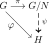
\includegraphics[width = 0.1\textwidth]{UniqueFactorTheorem.pdf}
		\caption{If $ N\nsg G $ and $ \varphi $ is any homomorphism such that $ N\subseteq \kernel \varphi $, then above is true.}
	\end{centering}
\end{figure}
\begin{proof}
	Consider the definition of a map $ \psi : A \to B $ as a set of ordered pairs $ (a,b) $. We need to show that for every $ a\in A $, there exists a $ b\in B $ such that $ (a,b) \in \psi $ and also that if $ (a_1,b_1),(a_2,b_2)\in \psi $ and $ a_1 = a_2 $, it implies that $ b_1 = b_2 $.\\
	Consider now $ x,y \in G$. If $ \inv{x}\cdot y \in N $ and since $ \kernel\varphi = N $, so $ \varphi(\inv{x}\cdot y) = \varphi(\inv{x})\cdot \varphi(y) = \inv{(\varphi(x))}\cdot \varphi(y) = 1$. Hence $ x\cdot N = y\cdot N $ implies that $ \varphi(x) = \varphi(y) $. In the form of the set of ordered pair, we can write,
	\[ \psi = \{(x\cdot N, \varphi(x))\;\vert\; x\in G\}. \]
	Now for $ \psi $ to be a map form $ G/N $ to $ H $, we already have that for every $ x\cdot N \in G/N $, there exists a $ \varphi(x) \in H $ and the second condition is proved as above. Hence $ \psi : G/N \to H $ is a map. Moreover, since $ \psi (x\cdot N) = \varphi(x) $, hence $ \varphi = \psi \circ \pi $. \\
	Uniqueness of $ \psi $ can be seen by assuming $ \xi : G/N \to H $ be another such homomorphism such that $ \xi \circ \pi = \varphi $. But then $ \xi (x\cdot N) = \varphi(x) = \psi(x\cdot N) $ for each $ x\cdot N \in G/N $ for each $ x\in G $. Hence $ \xi = \psi $.
\end{proof}
\hrulefill
\textbf{THE HOMOMORPHISM THEOREM}
\hrulefill
\begin{theorem}
	(\textbf{Homomorphism Theorem}) If $ \varphi : A \longrightarrow B $ is a homomorphism of groups, then
	\[A/\kernel \varphi \isomorph \image \varphi.\]
	That is, there is a unique isomorphism $ \theta : A/\kernel \varphi \to \image \varphi $ such that $ \varphi = \iota \circ \theta \circ \pi $ where $ \iota : \image f \to B $ is the inclusion homomorphism and $ \pi : A \to A/\kernel f $ is the canonical projection.
\end{theorem}
\begin{figure}[h!]
	\[
	\begin{tikzcd}
		A \arrow{r}{\varphi} \arrow[swap]{d}{\pi} &B \\
		A/\kernel \varphi \arrow[swap, dashed]{r}{\theta} &\image \varphi \arrow[swap]{u}{\iota}
	\end{tikzcd}
	\]
	\caption{If $ \varphi $ is any homomorphism, then above is true.}
\end{figure}

\begin{proof}
	Consider the homomorphism $ \psi : A \to \image \varphi $ to be equal to the map $ \varphi $. We have that $ \kernel \psi = \kernel \varphi $, moreover, from Theorem 1, we have that $ \psi = \theta \circ \pi $ for some unique homomorphism $ \theta : A/\kernel \varphi \to \image \varphi $. Denoting $ K = \kernel \varphi $, we get that $ \theta(a\cdot K) = \theta(a)\cdot\theta(K) = \psi(a) = \varphi(a) $ for all $ a\in A $. Hence $ \varphi = \iota \cdot \theta  \cdot \pi$. We can also see that $ \theta $ is a surjection (Proposition 23) and since $ \theta(a\cdot K) = 1 \implies \varphi(a) = 1 \implies a \in \kernel\varphi \in A/\kernel\varphi$, so $ \theta $ is injective, hence bijective. Theorem 1 also proves the uniqueness of $ \theta $.% consider another isomorphism $ \xi : A/\kernel \varphi \to \image \varphi $ such that $ \varphi = \iota \cdot \xi \cdot \pi $. In such a case, $ \xi (a\cdot K) = \varphi(a) = \theta(a\cdot K) $ for all $ a\in A $. Hence $ \xi = \theta $.
\end{proof}
\begin{corollary}
	If $ \varphi: A\to B $ is injective, then $ A\isomorph \image \varphi $ and if $ \varphi $ is surjective, then $ A/\kernel\varphi \isomorph B $.
\end{corollary}
\begin{proof}
	If $ \varphi $ is injective, then $ \kernel \varphi = 1 $ and if $ \varphi $ is surjective, then $ B = \image \varphi $.
\end{proof}
\begin{remark}
	Homomorphism theorem tells us that \emph{every homomorphism is a composition of an inclusion homomorphism of subgroups, an isomorphism and the canonical projection to quotient groups.}
\end{remark}
\hrulefill
\begin{proposition}
	Let $ G $ be a group and let $ a\in G $. If $ a^m \neq 1 $ for all $ m\neq 0 $, then $ \gen{a} \isomorph \mathbb{Z} $ and $ \gen{a} $ is infinite.\\\\
	Conversely, if there is a smallest positive integer $ n $ such that $ a^n = 1 $, then $ a^m = 1 $ if and only if $ n $ divides $ m $ and $ \gen{a} \isomorph \mathbb{Z}_n $ and order of $ \gen{a} $ is $ n $.
\end{proposition}
\begin{proof}
	Consider the homomorphism $f : m \to a^m $ from $ \mathbb{Z} $ to $ G $. By Theorem 2, we have that $ \mathbb{Z}/\kernel f \isomorph \image f = \gen{a} $. Since $ \kernel f $ is a subgroup of $ \mathbb{Z} $ and since every subgroup of $ \mathbb{Z} $ is cyclic, hence $ \kernel f $ is cyclic. Let $ n \in \kernel f $, therefore $ a^n = 1 $ and hence $ \kernel f = \mathbb{Z}\cdot n $ for some $ n $. If $ n=0 $, then $ \mathbb{Z} \isomorph \mathbb{Z}/0 \isomorph \gen{a} $. If $ n>0 $, we have that $ \gen{a} \isomorph \mathbb{Z}/\mathbb{Z}\cdot n = \mathbb{Z}_n $. Hence $ a^m = 1$ if and only if $ m $ is a multiple of $ n $ (Proposition 24).
\end{proof}
\hrulefill
\begin{definition}
	(\textbf{Order of an element of a group}) The order of an element $ a $ of a group $ G $ is infinite if $ a^m \neq 1 $ for all $ m\neq 0 $. Otherwise, the order of element $ a $ is the smallest positive integer $ n $ such that $ a^n = 1 $.
\end{definition}
\begin{corollary}
	Any two cyclic groups of order $ n $ are isomorphic.
\end{corollary}
\begin{proof}
	By Proposition 27, we have that any cyclic group of order $ n $ is isomorphic to $ \mathbb{Z}_n $, hence they are isomorphic to each other too (Proposition 16).
\end{proof}
\begin{corollary}
	Every subgroup of a cyclic group is cyclic.
\end{corollary}
\begin{proof}
	Let $ G $ be a cyclic group, therefore $ G = \gen{a} $ for some $ a\in G $. Let $ H\le \gen{a} $. This implies that $ a^m \in H $ for the smallest positive integer $ m\in \mathbb{Z} $. Now consider $ b\in H $, therefore $ b = a^n $ for some $ n\in \mathbb{Z} $. By division theorem, we can write $ n = mq + r $ where $ q,r \in \mathbb{Z} $ and $  0\le r < m$. Hence $ a^n = a^{mq+r} = a^{mq}a^r = (a^m)^q a^r$ which implies that $ a^r = (a^m)^{-q} a^n $. Since $ a^m \in H $, then $ \inv{(a^m)}\in H $ and so on, $ (a^m)^{-q} \in H$. Since $ a^n \in H $ too and $ H $ is a subgroup, hence $ a^r = (a^m)^{-q} a^n \in H$. But since $ r<m $ and $ a^r \in H $, it implies that $ r=0 $, hence $ a^n = (a^m)^q $, that is, $ H = \gen{a^m} $.
\end{proof}
\begin{remark}
	We denote the \emph{cyclic group of order} $ n $ by $ C_n $.
\end{remark}
\hrulefill
\textbf{THE ISOMORPHISM THEOREMS}
\hrulefill

We now discuss the next isomorphism theorems.
\begin{theorem}
	(\textbf{The First Isomorphism Theorem}) Let $ A $ be a group and let $ B,C $ be normal subgroups of $ A $. If $ C\subseteq B $, then $ C $ is a normal subgroup of $ B $, $ B/C $ is a normal subgroup of $ A/C $ and
	\[A/B \isomorph (A/C)/(B/C).\]
	In particular, there is a unique isomorphism $ \theta : A/B \to (A/C)/(B/C) $ such that $ \theta \circ \rho = \tau \circ \pi $ where $ \rho : A \to A/B $, $ \tau : A/C \to (A/C)/(B/C) $ and $ \pi : A\to A/C $. \\\\
	The following commutative diagram explains the situation in detail (note that we have also used the Theorem 1 to draw $ \sigma : A/C \to A/B$).
	\begin{figure}[h!]
			\[\begin{tikzcd}
			A \arrow{r}{\pi} \arrow[swap]{d}{\rho}&A/C \arrow[swap,dashed]{dl}{\sigma} \arrow{d}{\tau}\\
			A/B \arrow[swap,dashed]{r}{\theta} &(A/C)/(B/C)
		\end{tikzcd}\]
	\caption{Let $ B,C \nsg A $ with $ C\subseteq B $. Then $ C\nsg B $, $ B/C \nsg A/C $ and the above is true.}
	\end{figure}
\end{theorem}
\begin{proof}
	Since, $ C\nsg A $ and since $ C \subseteq B $, therefore $ C\nsg B $. By Theorem 1, we can factor $ \rho $ via a unique homomorphism $ \sigma : A/C \to A/B$ such that $ \rho = \sigma \circ \pi $. Therefore, for any $ b\cdot C \in A/C $ for $ b\in B $, we get $ \sigma(b\cdot C) = b\cdot B =B \in A/B $ (Proposition 12). Moreover, if $ \sigma(a\cdot C) = 1 = B $, then (Proposition 17, 1.) $ a\cdot B = B\implies a\in B$. Therefore, $ \kernel \sigma = \{b\cdot C\;\vert\; b\in B\} = B/C$. Also, since $ \kernel \sigma \nsg A/C$ (Proposition 19), thus, $B/C \nsg A/C$. By Theorem 2, we now have that $ (A/C)/(B/C) \isomorph \image \sigma$, but since for any $ a\cdot B \in A/B$, we have a $ a\cdot C \in A/C $ as $ C\subseteq B $, therefore $ \image \sigma = A/B $ and hence $ (A/C)/(B/C) \isomorph A/B $. Theorem 2 also proves the uniqueness of this isomorphism.
\end{proof}
\hrulefill
\newpage
\begin{theorem}
	(\textbf{The Second Isomorphism Theorem}) Let $ A $ be a subgroup of a group $ G $ and let $ N $ be a normal subgroup of $ G $. Then $ A\cdot N $ is a subgroup of $ G $, $ N $ is a normal subgroup of $ A\cdot N $, $ A\cap N $ is a normal subgroup of $ A $ and 
	\[(A\cdot N) / N \isomorph A/(A\cap N).\]
	In particular, there is a unique isomorphism $ \theta : A/(A\cap N) \to (A\cdot N) / N $ such that $ \theta \circ \rho = \pi \circ \iota $ where $ \rho : A\to A/(A\cap N)$, $ \pi : A\cdot N \to (A\cdot N)/N $ are the canonical projections and $ \iota : A \to  A\cdot N $ is the inclusion homomorphism.
	\begin{figure}[h!]
		\[\begin{tikzcd}
			A \arrow{r}{\rho} \arrow[swap]{d}{\iota} \arrow[swap]{dr}{\varphi} &A/(A\cap N) \arrow[dashed]{d}{\theta}\\
			A\cdot N \arrow[swap]{r}{\pi} &(A\cdot N)/N
		\end{tikzcd}\]
	\caption{Let $ A \le G $, $ N\nsg G $. Then $N\nsg A\cdot N \le G$, $ A\cap N \nsg A $ and the above is true. }
	\end{figure}
\end{theorem}
\begin{proof}
	First, note that $ A\cdot N = \{a\cdot n\;\vert\; a\in A, \;n\in N\} $ (Definition 7). Since $ 1\in A $ and $ 1 \in N$, hence $ 1\in A\cdot N $. For $ x \in A\cdot N \implies x= a\cdot n$ for some $ a\in A,\;n\in N $. Note that $ \inv{a}\in A $ and $ \inv{n}\in N $ which implies that $ \inv{n}\cdot \inv{a}\in N\cdot A = N\cdot A$ ($ N $ is normal). Hence $\inv{x}= \inv{(a\cdot n)} = \inv{n}\cdot \inv{a} \in A\cdot N $. Also, for $ a_1,a_2 \in A $ and $ n_1,n_2 \in N $, we get that $ a_1\cdot n_1, a_2\cdot n_2 \in N $, hence $ a_1\cdot n_1 \cdot a_2\cdot n_2 = (a_1\cdot a_2)\cdot n_1\cdot n_2 = (a_1\cdot a_2 )\cdot n_3 \in A\cdot N$ for some $ n_3 = n_1\cdot n_2 \in N $. Hence $ A\cdot N \le G$. \\
	Clearly, $ 1\in N $ as $ N\nsg G $ and by Proposition 10 we get $ N\nsg A\cdot N $.\\
	So far, we have that $ N\nsg A\cdot N \le G$ and trivially, $ N \subseteq A\cdot N $. Also, from Proposition 10, $ N\le G $. Consider now the homomorphism $ \varphi = \pi \circ \iota $ (Theorem 1). Now, for some $ a\in A $, we get $ \varphi(a) = (a\cdot N)/N = N\cdot a\cdot N = a\cdot N$. Hence, if $ a\in A\cap N $, then $ a\cdot N = N =1\varphi(a) $. Conversely, $ \varphi(A\cap N) = ((A\cap N )\cdot N)/N = (A\cdot N \cap N)/N = (A\cdot N)/N$. Hence $ \kernel \varphi = A\cap N $. Now using Theorem 2, we get that $ A/\kernel \varphi = A/(A\cap N) \isomorph \image \varphi$. Since $ \image \varphi = \varphi(A) = (A\cdot N)/N $, hence $ A/(A\cap N) \isomorph (A\cdot N)/N $ uniquely. 
\end{proof}
\hrulefill
\newpage
\subsection{The Direct Products}
These are an easy way to construct larger groups from smaller ones. \emph{This construction yields all \textbf{finite abelian groups}}.

\hrulefill
\begin{definition}
	(\textbf{Direct Product}) The direct product of two groups $ G_1 $ and $ G_2 $ is their Cartesian Product $G_1 \times G_2 $ also denoted by $G_1 \oplus G_2$, together with the component-wise operation $ (\cdot) $. That is, for $ x_1,y_1 \in G_1 $ and $ x_2,y_2\in G_2 $, we have $ (x_1,x_2), (y_1,y_2) \in G_1\oplus G_2 $ and
	\[(x_1,x_2)\cdot (y_1,y_2) = (x_1\cdot y_1,x_2\cdot y_2) \in G_1\oplus G_2.\]
\end{definition}
\begin{remark}
	Note that $ G_1\oplus G_2 $ is also a group.
	\begin{itemize}
		\item{Associativity of $ G_1\oplus G_2 $ can be seen by the associativity of $ G_1 $ and $ G_2 $:
	\begin{equation*}
		\begin{split}
			(x_1,x_2)\cdot \left((y_1,y_2) \cdot (z_1,z_2) \right) = (x_1,x_2)\cdot (y_1\cdot z_1,y_2\cdot z_2) &= (x_1\cdot y_1\cdot z_1, x_2\cdot y_2\cdot z_2) \\
			&= ((x_1\cdot y_1)\cdot z_1, (x_2\cdot y_2)\cdot z_2)\\
			&= ((x_1,x_2)\cdot (y_1,y_2))\cdot (z_1,z_2)
		\end{split}
	\end{equation*}	
	}
\item{Since $ (1_{G_1}, 1_{G_2})\in G_1\oplus G_2$, hence, for any $ (x,y) \in G_1\oplus G_2 $, we see the following:
\[(1_{G_1}, 1_{G_2}) \cdot (x,y) = (1_{G_1}\cdot x, 1_{G_2} \cdot y) = (x\cdot 1_{G_1}, y\cdot 1_{G_2}) = (x,y)\cdot(1_{G_1}, 1_{G_2}) =(x,y)\]
Hence, $ (1_{G_1},1_{G_2}) $ is the Identity of $ G_1\oplus G_2 $ under $ (\cdot) $.
}
\item{For any $ (x,y)\in G_1 \oplus G_2$, we have $ (\inv{x},\inv{y}) \in G_1\oplus G_2$ because $ G_1 $ and $ G_2 $ are also groups and they contain inverse of each element. Hence, 
\[(x,y)\cdot (\inv{x},\inv{y}) = (x\cdot \inv{x}, y\cdot\inv{y}) = (1_{G_1}, 1_{G_2}).\]
}
	\end{itemize}
\end{remark}
\hrulefill
\textbf{DIRECT SUMS}
\hrulefill

\emph{The conditions under which a group splits into a direct product.}
\begin{proposition}
	A group $ G $ is isomorphic to the direct product $ G_1\oplus G_2 $ of two groups $ G_1 $ and $ G_2 $ if and only if it contains normal subgroups $ A\isomorph G_1 $ and $ B\isomorph G_2 $ such that $ A\cap B = 1$ and $ A\cdot B = G $.
\end{proposition}
\hrulefill
\begin{definition}
	(\textbf{Direct Sum}) A group $ G $ is the internal direct sum $ G = A\oplus B $ of two subgroups $ A $ and $ B $ when $ A,B \nsg G $, $ A\cap B = 1 $ and $ A\cdot B = G $.
\end{definition}
\begin{remark}
	Note that the conditions for a group $ G $ to be broken down into direct products is rather stringent. This however leads to easier results in Abelian Groups as shown next.
\end{remark}
\hrulefill
\begin{theorem}
	Every finite abelian group is isomorphic to the direct product of cyclic groups whose orders are positive powers of prime numbers and these cyclic groups are unique, up to order of appearance and isomorphism.
\end{theorem}
\begin{remark}
	This theorem implies that any abelian $ p $-group of order $ p^k $ is hence isomorphic to the direct product of cyclic groups as $ C_{p^{k_1}}\oplus C_{p^{k_2}} \oplus \dots \oplus C_{p^{k_r}} $ where $ k_1 + \dots + k_r = k $. \\
	We also have the following easy corollary.
\end{remark}
\begin{corollary}
	Let $ p_1,\dots,p_r $ be distinct primes. An abelian group of order $ p_1^{k_1}p_2^{k_2}\dots p_r^{k_r} $ is a direct sum of subgroups of orders $ p_1^{k_1},p_2^{k_2},\dots, p_r^{k_r}  $
\end{corollary}
\hrulefill
All Abelian Groups of order $ n $
\hrulefill

We can now find all abelian groups of order $ n $ as follows.
\begin{enumerate}
	\item {Write $ n $ as a product of positive powers $ p^k $ of distinct primes.}
	\item {For each $ p $, find all abelian $ p $-groups of order $ p^k $ from the partitions of $ k $.}
	\item {The abelian groups of order $ n $ are the direct products of these $ p $-groups, one for each prime divisor $ p $ of $ n $.}
\end{enumerate}
Consider example of $ n = 200 = 2^3\cdot 5^2 $. We need to find now the partitions of $ 3 $ and $ 2 $. There are three partitions of 3 : $ 1+1+1, 2+1, 3+0 $. There are two partitions of 2 : $ 1+1, 2+0 $. Hence there are three cyclic groups of order 8 : $ C_2\oplus C_2\oplus C_2\;;\;\;C_4\oplus C_2 \;;\;\;C_8$ and there are 2 cyclic groups of order $ 25 $ : $ C_5\oplus C_5\;;\;\;C_{25} $. Finally, there would be $ 3\times 2 = 6$ abelian groups of order 200, each of which would be a combination of the two sets of the groups above.

\hrulefill
\begin{proposition}
	If $ m $ and $ n $ are relatively prime, then
	\[C_{mn} \isomorph C_{m}\oplus C_{n}\]
\end{proposition}
\begin{remark}
	Hence $ C_2\oplus C_2 \oplus C_2 = C_2\oplus C_4 = C_8 $ and similarly for others in the above example.
\end{remark}
\newpage
\hrulefill
\textbf{EULER'S $ \phi $ FUNCTION}
\hrulefill
\begin{definition}
	(\textbf{Euler's function}) Euler's function $ \phi(n) $ is the number of integers $ 1\le k\le n $ that are relatively prime to $ n $. That is, it is the cardinality of the set
	\[\phi(n) = \abs{\{a  \;\vert\; \gcd(a,n) = 1\}}\]
\end{definition}
\begin{remark}
	We have:
	\begin{itemize}
		\item {If $ p $ is prime, then $ \phi(p) = p-1 $.}
		\item {If $ n= p^m $, then $ \phi(p^m) = p^m - (p^m/p)  = p^m\left (1-\frac{1}{p}\right )$ since every $ p^{th} $ number is a multiple of $ p^m $.}
	\end{itemize}
\end{remark}
\hrulefill
\begin{proposition}
	A cyclic group of order $ n $ has exactly $ \phi(n) $ elements of order $ n $.
\end{proposition}
\begin{proof}
	Let $ G  = \gen{c}$ be a cyclic group of order $ n $. Let $ 1\le k\le n $ and then $ c^k \in \gen{c} $. Clearly, the order of the element $ c^k $ divides $ n $, by Lagrange's Theorem. Now, assume that $ \gcd(n,k) = d>1 $. Then $ (c^k)^{n/d} = 1$. But then, this implies that order of $ c^k $ is atmost $ n/d < n$. Whereas, if $ \gcd(n,k) = 1 $, then $ (c^k)^m = 1$ implies that order of $ c $ is $ km $, but since order of $ c $ is $ n $, hence $ n $ divides $ km $ and since $ n $ and $ k $ are relatively prime, therefore $ n $ divides $ m $. Hence $ c^k $ has order $ n $ only when $ \gcd(n,k) = 1 $, so that there are $ \phi(n) $ such elements of order $ n $.
\end{proof}
\hrulefill

\emph{SUBTRACT TWO PROPOSITIONS, ONE COROLLARY \& ONE DEFINITION FROM EVERY REF. BELOW.}
\newpage
\subsection{Group Actions}
\begin{definition}
	(\textbf{Group Action}) A left group action of a group $ G $ on a set $ X $ is a mapping $ G\times X \to X $ or $ (g,x)\to g\cdot x $ such that
	\begin{enumerate}
		\item{$ 1\cdot x = x $.}
		\item{$ g\cdot(h\cdot x) = (g\cdot h)\cdot x$ for all $ g,h\in G $ and $ x\in X $.}
	\end{enumerate}
Then $ G $ is said to be \emph{acting on the left of $ X $}.
\end{definition}
\begin{remark}
	We can similarly define the \emph{right group action.}
\end{remark}
\hrulefill
\textbf{PROPERTIES}
\hrulefill
\begin{proposition}
	In a left group action of a group $ G $ on a set $ X $, the action $ \sigma_g : x \to g\cdot x $ of $ g\in G $ is a permutation of $ X $. Moreover, $ g\to \sigma_g $ is a homomorphism of $ G $ into the symmetric group $S_X $.
\end{proposition}
\begin{proof}
	First note that $ \sigma_g \circ \sigma_h : x\to (g\cdot h) \cdot x$ and hence $ \sigma_g \circ \sigma_{\inv{g}} = 1_X = \sigma_{\inv{g}} \circ \sigma_g $ which implies that $ \sigma_g $ is a bijection from $ X $ to $ X $. Now since $ \sigma_{g\cdot h} = \sigma_g \circ \sigma_h $, hence $ g \to \sigma_g $ is a homomorphism.
\end{proof}
\begin{remark}
	The symmetric group on a finite set $ X $ is the group whose elements are all bijective functions from $ X $ to $ X $ and whose group operation is that of function composition.
\end{remark}
\hrulefill
\begin{proposition}
	There is a one-to-one correspondence between left actions of $ G $ on $ X $ and homomorphisms $ G\to S_X $.
\end{proposition}
\begin{proof}
	The left actions of $ G $ on $ X $ are the action maps $ \sigma_g : x \to g\cdot x$ for all $ g\in G $. Also, the homomorphisms from $ G\to S_X $ are maps $ \rho_g : g \to \sigma_g $. Now for each unique $ g\in G $, we have a corresponding $ \sigma_g $ and hence the corresponding $ \rho_g $. Similarly, for each $ \rho_g $, we have a unique $ \sigma_g $. Hence the bijection between left actions and homomorphisms $ G\to S_X $.
\end{proof}
\hrulefill
\begin{theorem}
	(\textbf{Cayley's Theorem}) Every group $ G $ is isomorphic to a subgroup of the symmetric group $ S_G $.
\end{theorem}
\begin{proof}
	Let $ G $ act on $ G $ itself by left group action. Therefore $ \sigma : G \to S_G $ is a permutation of $ G $ and hence an injection (Proposition 29). Moreover, $\sigma $ is also a surjection from $ G $ to $ \image \sigma $. Hence $ G \isomorph \image \sigma \le S_G$.
\end{proof}
\hrulefill
\begin{proposition}
	Let the group $ G $ act on the left of a set $ X $. The relation 
	\[x\equiv y \;\text{if and only if}\;y=g\cdot x\;\text{for some }g\in G\]
	is an equivalence relation on $ X $.
\end{proposition}
\begin{proof}
	Since $ G $ acts on set $ X $ hence for $ 1\in G $, we have $ 1\cdot x = x $, hence $ x\equiv x $. For $ y\equiv x$, we have $ y= g\cdot x \implies x = \inv{g}\cdot x$ and since $ \inv{g}\in G $ hence $ x\equiv y $. Let $ x\equiv y $ and $ y\equiv z $, hence $ x = g_1\cdot y $ and $ y = g_2\cdot z $ for some $ g_1,g_2\in G $. We hence get $ x = g_1 \cdot (g_2\cdot z) = (g_1\cdot g_2)\cdot z$ due to the property of Group Action, and since $ g_1\cdot g_2 \in G $ too, therefore, $ x\equiv z $. Hence $ \equiv $ is an equivalence relation on $ X $.  
\end{proof}
\hrulefill
\begin{definition}
	(\textbf{Orbit}) In a left group action of a group $ G $ on a set $ X $, the orbit of $ x\in X $ is
	\[\{y\in X\;\vert \; y = g\cdot x \;\text{for some }g\in G\}\]
\end{definition}
\begin{remark}
	Therefore \emph{the orbit of $ x\in X $ are all those elements in $ X $ to which $ x $ can be moved to by the group action of $ G $.}\\
	Also, by virtue of Proposition 31, \emph{the different orbits of the elements of $ X $ constitute a partition of $ X $.}
\end{remark}
\hrulefill

We now look at the size of the orbits.
\begin{definition}
	(\textbf{Stabilizer}) In a left group action of a group $ G $ on a set $ X $, the stabilizer $ S(x) $ of $ x\in X $ is the following subgroup of $ G $:
	\[S(x) = \{g\in G\;\vert\; g\cdot x = x\}\]
\end{definition}
\newpage
\hrulefill
\begin{proposition}
	The order of the orbit of an element is equal to the index of it's stabilizer.
\end{proposition}
\begin{proof}
	Let $ G $ be a group acting on a set $ X $. For some $ x\in X $, consider the map $ g\to g\cdot x $ from $ G $ to orbit of $ X $. Clearly, this is a surjection. Moreover, notice that this map induces a bijection between the elements of orbit of $ x $ and the equivalence classes of group $ G $ induced by this map. Note that equivalence class of $ G $ by this map is $ g\cdot x = h\cdot x \implies x = \inv{g}\cdot h \cdot x $ and hence $ \inv{g}\cdot h \in S(x)  $, hence the equivalence class here is the left cosets of $ S(x) $. Hence we have a bijection from left cosets of $ S(x) $ and the orbit of an element of $ X $.
\end{proof}
\hrulefill
\textbf{ACTION BY INNER AUTOMORPHISMS}
\hrulefill
\begin{proposition}
	For every element $ g $ of a group $ G $, the mapping $ \alpha_g : x\to g\cdot x\cdot \inv{g} $ for any $ x\in G $ is an automorphism of $ G $. Moreover, $ g \to \alpha_g $ is a homomorphism of $ G $ into $ \Auto{G} $.
\end{proposition}
\begin{proof}
	Remember that an automorphism is a bijective homomorphism from $ G $ to $ G $. First note that for $ x,y \in G $, we have $ \alpha_g(x\cdot y) = g\cdot (x\cdot y)\cdot \inv{g} = g\cdot (x\cdot \inv{g}\cdot g\cdot y)\cdot \inv{g} = (g\cdot x\cdot \inv{g})\cdot (g\cdot y\cdot \inv{g})$ hence $ \alpha_g $ is an endomorphism. For injection, consider $ \alpha_g(x) = \alpha_g(y) $ for $ x,y\in G $. We get that $ g\cdot x\cdot \inv{g} = g\cdot y\cdot \inv{g} \implies x = y$ by cancellation law (Proposition 1). For surjection, note that $ \alpha_g \circ \alpha_{\inv{g}} = \text{Id}_G = \alpha_{\inv{g}}\circ \alpha_g$, that is, we have $ \alpha_g $ and $ \alpha_{\inv{g}} $ as mutually bijective inverses of each other. Hence $ \alpha_G $ is an automorphism. Also since under the map $ g\to \alpha_g $, we have that $ g\cdot h \to \alpha_{g\cdot h} =\alpha_g \circ \alpha_h $, hence $ g\to \alpha_g $ is a homomorphism from $ G $ to $ \Auto{G} $.
\end{proof}
\hrulefill
\begin{definition}
	(\textbf{Inner Automorphism}) An inner automorphism of a group $ G $ is an automorphism $ x\to g\cdot x\cdot \inv{g} $ for some $ g\in G $.
\end{definition}
\hrulefill
\begin{definition}
	(\textbf{Action by Inner Automorphism}) The action of a group $ G $ on itself by inner automorphism is defined by:
	\[g\bullet x = g\cdot x\cdot \inv{g}\;\;\text{for all} \;g,x\in G\]
	and we denote $ g\cdot x\cdot \inv{g} $ by $ ^gx $.
\end{definition}
\begin{remark}
	$ g\bullet x = g\cdot x\cdot \inv{g} $ is indeed a group action.
\end{remark}
\hrulefill
\begin{definition}
	(\textbf{Conjugacy Class}) In the action of a group $ G $ on itself by inner automorphisms, the orbits are the conjugacy classes of $ G $. 	Moreover, two elements are conjugate when they belong to the same conjugacy class.
\end{definition}
\begin{remark}
	More simply, two $ x,y\in G $ are said to be \emph{conjugate} in $ G $ when $ y = g\cdot x\cdot \inv{g} $ for some $ g\in G $.\\
	By Proposition 31, \emph{conjugacy is an equivalence relation}.
\end{remark}
\hrulefill
\begin{definition}
	(\textbf{Center of a Group}) The center of a group $ G $ is 
	\[Z(G) = \{g \in G\;\vert\; g\cdot x\cdot \inv{g} = x \;\;\text{for all}\;x\in G\}.\]
\end{definition}
\begin{remark}
	Hence, the conjugacy class of $ x $ is said to be \textbf{\textit{trivial}}, that is $ g\cdot x\cdot \inv{g} = x$ for all $ x \in G$, if and only if $ x $ lies in the center of $ G $. We can see this by noticing that $ Z(G) = \{g\in G\;\vert\; g = x\cdot g\cdot \inv{x}\;\;\text{for all}\;x\in G\} $.
\end{remark}
\hrulefill
\begin{proposition}
	$ Z(G) $ and all of it's subgroups are normal subgroups of $ G $.
\end{proposition}
\begin{proof}
	Consider $ z\in Z(G) $. This implies that $ z\cdot x\cdot \inv{z} = x \implies z\cdot x = x\cdot z$ for all $ x\in G $. Now for any $ g\in G $, we hence have $ g\cdot z = z\cdot g$. Therefore $ g\cdot H = H\cdot g $ for all $ g $ and $ H\le Z $, that is $ H \nsg G$.
\end{proof}
\hrulefill
\begin{definition}
	(\textbf{Centralizer of an Element}) The centralizer in $ G $ of an element $ x $ of a group $ G $ is
	\[C_G(x) = \{g\in G\;\vert\;g\cdot x \cdot \inv{g} = x\}.\]
\end{definition}
\hrulefill
\begin{proposition}
	The number of conjugates of an element of a group $ G $ is the index of it's centralizer in $ G $.
\end{proposition}
\begin{proof}
	Note that the number of conjugates of an element is the order of it's conjugacy class. Since the conjugacy class of an element in $ G $ is just it's orbit when $ G $ acts by inner automorphism, hence the  order of conjugacy class is equal to the index of stabilizer of that element (Proposition 32). But the stabilizer in the case of inner automorphism is just the centralizer. Hence number of conjugates of an element in $ G $ is the number of left cosets of it's centralizer.
\end{proof}
\hrulefill
\textbf{CLASS EQUATION}
\hrulefill
\begin{proposition}
	(\textbf{The Class Equation}) In a \textbf{finite group} $ G $, we have the following,
	\begin{equation}\label{ClassEquation}
		\boxed{\order{G} = \sum \order{C} = \order{Z(G)} + \sum_{\order{C}>1}\order{C}}
	\end{equation}
	The first sum has one term for each conjugacy class $ C $ and the second sum has one term for each non-trivial conjugacy class $ C $.
\end{proposition}
\begin{proof}
	Since the conjugacy classes forms a partition of $ G $ by Proposition 31, hence $  \order{G} = \sum \order{C}$. But there are certain trivial conjugacy classes (whose order is 1) and they are the classes of members of center of the group $ G $. Hence we have $ \order{Z(G)} $ number of trivial conjugacy classes. Therefore the order of the group can be written as the sum of these $ \order{Z(G)} $ trivial classes and all other non-trivial classes.  
\end{proof}
\hrulefill
\begin{definition}
	(\textbf{$ p $-groups}) A $ p $-group is a group whose order is a power of a prime $ p $. 
\end{definition}
\begin{remark}
	The class equation yields interesting properties of these groups.
\end{remark}
\hrulefill
\begin{proposition}
	Every non-trivial $ p $-group has a non-trivial center.
\end{proposition}
\begin{proof}
	Consider $ G $ to be a $ p $-group so that $ \order{G} = p^k $ for some $ k>0 $. Now assume that $ G $ has a trivial center ($ Z(g) = \{1_G\} $). Therefore by Class Equation (Proposition 36), we have that $ p^{k}=\sum \order{C} = 1 + \sum_{\order{C}>1} \order{C} $. Now by Lagrange's Theorem (Proposition 15), Proposition 35 and the observation that centralizer of an element in $ G $ is a subgroup of $ G $, we can say that $ \order{C} $ divides $ \order{G} = p^k$ apart from the case when $ \order{C} = 1 $. Hence we can write class equation as 
	\[p^k = 1 + p \times (n_1 + n_2 + \dots) = 1+ pn \;\text{for some}\;n>0\]
	which implies that $ p^{k-1} = \frac{1}{p} + n $, and since $ p $ is a prime, we have a contradiction. Hence every non-trivial $ p $-group has a non-trivial center. 
\end{proof}
\hrulefill
\begin{proposition}
	Every group of order $ p^2 $ where $ p $ is prime is abelian.
\end{proposition}
\begin{proof}
	Consider a group $ G $ of order $ p^2 $. Proposition 37 yields that $ \order{Z(G)} > 1 $ and Class Equation yields (or for that matter, Lagrange's Theorem) that $ \order{Z(G)} = p $ or $ \order{Z(G)} = p^2 $. For $ \order{Z(p)} = p^2 $, we would from Class Equation and Proposition 31 have that $ G =  Z(G)$ and since $ Z(G) $ is commutative, hence $ G $ would also be commutative. \\
	Next, if $ \order{Z(G)} = p $, then the quotient group $ G/Z(G) $ would also have order $ p $ by Lagrange's Theorem. Since any group of order $ p $ is cyclic (Lagrange's theorem implies that any subgroup has to be trivial), which further implies that if $ G/Z(G) $ is cyclic, then for some $ g_1\cdot Z(G) \in G/Z(G) $ and for any $ g_2\cdot Z(G) \in G/Z(G) $ it is true that $ g_2\cdot Z(G) = \left( g_1\cdot  Z(G)\right )^m $ for some $ m >0$. Expanding this yields us, 
	\begin{equation*}
		\begin{split}
			g_2\cdot Z(G) &= g_1\cdot Z(G)\cdot g_1\cdot Z(G) \;\dots \; g_1\cdot Z(G)\\
			&= g_1^m\cdot Z(G)^m \;\;\;\;\;\;\text{(Since $ Z(G) $ is Normal, Proposition 34)}\\
			&= g_1^m\cdot Z(G) \;\;\;\;\;\;\text{(Since $ Z(G) $ is the set of commuting elements of $ G $)}\\
		\end{split}
	\end{equation*} 
which implies by cancellation law of groups that $ g_2 = g_1^m $ for any $ g_2\in G $ and for some $ g_1\in G $ and corresponding $ m>0 $. Similarly, for $ g_3\in G $, we would have $ g_3 = g_1^n $. Hence $ g_3\cdot g_2 = g_1^n\cdot g_1^m = g_1^{n+m} = g_1^{m+n} = g_1^m\cdot g_1^n = g_2\cdot g_3 $. Hence $ G $ is commutative in this case too.
\end{proof}
\hrulefill
\newpage
\subsection{The Sylow Theorems}
These are a basic tool in finite Group Theory. They are existence theorems of certain subgroups.

\hrulefill

First theorem is a \emph{partial converse of Lagrange's Theorem}.
\begin{theorem}
	(\textbf{First Sylow Theorem}) Let $ G $ be a \textbf{finite group} and let $ p $ be a prime number. If $ p^k $ divides the order of $ G $, then $ G $ has a subgroup of order $ p^k $.
\end{theorem}
\begin{proof}
%	\textit{Add proof later.}
We first prove that \emph{If $ G $ is abelian and $ p $ divides $ \order{G} $, then $ G $ has a subgroup of order $ p $.}\\\\
For this, first consider that $ \order{G} = p$, then $ G \nsg G$ will do. Next, for $ \order{G}>p $, we proceed by induction on $ \order{G} $. Let $ a\in G $ such that $ a\neq 1 $. Now if order of $ a $ is a multiple of $ p $, as $ mp $, then we have a subgroup $ \gen{a} $ whose order is divided by $ p $ and then we would be done. But if we have order of $ a $ not a multiple of $ p $, then it should be true that index of $ \gen{a} $, equivalently, the order of $ G/A $ must be divisible by $ p $. By induction, there would be an element of $ G/A $ whose order would be divisible by $ p $, let that element be $ b\cdot A $ for some $ b\in G $. Notice that order of $ b\cdot A $ would be $ k $ such that $ (b\cdot A)^k = b^k \cdot A^k= b^k \cdot A= A $ in $ G/A $. This implies that $ k $ must be a multiple of order of $ b $. But since $ k $ is divided by $ p $, hence order of $ b $ is divided by $ p $. Therefore, $ \gen{b}\le G $ is a subgroup whose order is divisible by $ p $, hence, by induction, $ G $ has a subgroup of order $ p $.\\
\emph{Note that we used abelian nature of $ G $ in interpreting $ G/A $, as any subgroup of an abelian group is normal.}\\\\
Now let $ G $ be any finite group. We would still proceed by induction. If $ \order{G} = 1$, then this theorem is trivial. For $ \order{G}>1 $, we will prove by induction on $ \order{G} $ that if $ p^k $ divides $ \order{G} $, then there is a subgroup of $ G $ with order $ p^k $.\\\\
Consider the order of the center of $ G $, that is $ \order{Z(G)} $. First consider the case : If $ p $ divides $ \order{Z(G)} $, then $ Z(G) $ has a subgroup $ A $ of order $ p $ because $ Z(G) $ is by definition abelian. Therefore $ A \nsg G$ is a subgroup of order $ p $. Now, if it is the case that $ p^k $ divides $ \order{G} $ hence $ p^{k-1} $ divided $ \order{G} $, then clearly, $ p^{k-1} $ divides $ \order{G/A} <\order{G} $ by Lagrange's Theorem. By Induction, there is a  subgroup $ B/A \le G/A$ whose order is $ p^{k-1} $ and $ B $ has order $ p^k $ where $ B\le A\le G $ and then we are done.\\
Now for the second case : If $ p $ does not divide $ \order{Z(G)} $. But since $ \order{G} $ is divided by $ p^k $, then by Class Equation we get that $ \sum_{\order{C}>1} \order{C}$ cannot be divided by $ p $. That is, there is a atleast one non-trivial conjugacy class $ C $ such that $ p $ does not divide $ \order{C} $. Now, by Proposition 35, we have that the order of the conjugacy class $ C $ is the index of centralizer in $ G $ of any element of $ C $. That is, $ \order{C} = [G:C_G(x)] $ for any $ x\in C $. Hence we have $ \order{C} = [G:C_G(x)] \le \order{Z(G)} $ because $ C_G(x) \le Z(G)$. But since $ p $ does not divide $ \order{Z(G)} $, therefore atleast one $ \order{C} $ cannot be divided by $ p $, but $ \order{Z(G)} + \order{C} $ is surely divided by $ p $. We then have that $ \order{C} = \order{G} / \order{C_G(x)}$ is not divided by $ p $ but since $ \order{G} $ is divided by $ p^k $, hence $ \order{C_G(x)} < \order{G} $ is divided by $ p^k $. By induction, there is a subgroup of $ C_G(x) $ which has order $ p^k $.
\end{proof}
\begin{remark}
	Because being divisible by $ p^k $ means it is divisible by $ p^j $ for $ 0\le j\le k $, hence $ G $ also has atleast one subgroup each of order $ p^j $ for all $0 \le j \le k$.
\end{remark}
\hrulefill
%\newpage
\begin{corollary}
	(\textbf{Cauchy's Theorem}) A finite group whose order is divisible by a prime $ p $ contains an element of order $ p $.
\end{corollary}
\begin{corollary}
	Let $ p $ be a prime number. The order of a finite group $ G $ is a power of $ p $ if and only if the order of every element of $ G $ is a power of $ p $.
\end{corollary}
\hrulefill
\textbf{NORMALIZERS}
\hrulefill

Next Sylow Theorems are proved by allowing $ G $ act on it's subgroups by inner automorphisms.
\begin{definition}
	(\textbf{Conjugacy Classes of Subgroups}) In the action by inner automorphisms of a group $ G $ on it's subgroups, the orbits are the conjugacy classes of subgroups of $ G $. That is, two subgroups of $ G $ are conjugate when the belong to the same conjugacy class.
\end{definition}
\begin{remark}
	Thus, two subgroups $ H $ and $ K $ are \emph{conjugate} when $ K = g\cdot H \cdot \inv{g} $ for some $ g\in G $.\\
	Also, by extension of Proposition 32, \emph{the number of conjugates of a subgroup is the index of it's stabilizer.} 
\end{remark}
\hrulefill
\begin{definition}
	(\textbf{Normalizer of a Subgroup}) The normalizer in $ G $ of a subgroup $ H $ of $ G $ is the \emph{extension of centralizers but for subgroups} as shown:
	\[N_G(H) = \{g\in G\;\vert\;g\cdot H\cdot \inv{g} = H\}.\]
\end{definition}
\hrulefill
\begin{proposition}
	The number of conjugates of a subgroup of a group $ G $ is the index of it's normalizer in $ G $.
\end{proposition}
\hrulefill
\textbf{II$ ^{\text{\textbf{nd}}} $ and III$ ^{\text{\textbf{rd}}} $  THEOREMS}
\hrulefill

These theorems give \emph{properties of $ p $-subgroups of maximal order.}
\begin{definition}
	(\textbf{Sylow $ p $-subgroup}) Let $ p $ be prime. A Sylow $ p $-subgroup of a \textbf{finite group} $ G $ is a subgroup of order $ p^k $, where $ p^k $ divides $ \order{G} $ and $ p^{k+1} $ does not divide $ \order{G} $.
\end{definition}
\begin{remark}
	Note that First Sylow Theorem guarantees the existence of Sylow $ p $-subgroup.
\end{remark}
\hrulefill
\begin{proposition}
	If a Sylow $ p $-subgroup of a finite group $ G $ is normal in $ G $, then it is the largest $ p $-subgroup of $ G $ and the only Sylow $ p $-subgroup of $ G $.
\end{proposition}
\begin{proof}
	Consider $ S\nsg G $ to be the normal Sylow $ p $-subgroup of $ G $ of order $ p^{k_1} $. Now assume that $ T $ is a $ p $-subgroup of $ G $ of order $ p^{k_2} $ such that $ S\le T $. Clearly, we have that $ \order{S} = p^{k_1} \le p^{k_2} = \order{T} $ so that $ \order{T\cap S} = \order{S} = p^{k_1} $. By Theorem 4, $ S\nsg T\cdot S $, $ T\cap S \nsg T $ and $ T/(T\cap S) \isomorph (T\cdot S)/S $. Therefore, $ \order{T}/\order{T\cap S} = \order{T\cdot S}/\order{S} \implies \order{T} = \order{T\cdot S}\ge \order{S}$. Now, by the choice of $ S $, we have that $ \order{T\cdot S} = \order{S} $ which implies that $ T\subseteq T\cdot S = S $.\textbf{HELP!}
\end{proof}
\hrulefill
\begin{theorem}
	(\textbf{Second Sylow Theorem}) Let $ p $ be a prime number. The number of Sylow $ p $-subgroups of a finite group $ G $ divides the order of $ G $ and is congruent to 1 \textit{modulo} $ p $.
\end{theorem}
\begin{theorem}
	(\textbf{Third Sylow Theorem}) Let $ p $ be a prime number. All Sylow $ p $-subgroups of a finite group are conjugate.
\end{theorem}
\begin{proof}
%	\textit{Add proof later.}
To Prove : Number of Sylow $ p $-subgroups is congruent to 1 $ (\mod p) $.
\begin{enumerate}
	\itemsep-0.3em
	\item{Let $ S $ be a Sylow $ p $-subgroup.}
	\item{Clearly, the conjugates of $ S $ are also Sylow $ p $-subgroups by definition.}
	\item{Hence $ S $ acts on the set $ \mathcal{S} $ of all Sylow $ p $-subgroups by inner automorphisms.}
	\item{Under the action of $ S $ by inner automorphisms on $ \mathcal{S} $, the set $ \{S\} $ is the orbit of $ S $ because $ a\cdot S\cdot \inv{a} = S $ for all $ a\in S $ (Definitions 34 \& 35).}
	\item{Conversely, assume $ \{T\} $ is the trivial orbit of $ S $ under inner automorphism of $ S $ on $ \mathcal{S} $. This means that $ T = a\cdot T\cdot \inv{a} $ for all $ a \in S$.}
	\item{This implies that $ S \subseteq N_G(T) $. }
	\item{But then it means that $ S $ is normal in $ N_G(T) $.}
	\item{Hence, by Proposition 40, $ S $ is the largest and only Sylow $ p $-subgroup in $ N_G(T) $.}
	\item{But $ T $ is the trivial orbit, then it is also a Sylow $ p $-subgroup, hence $ S=T $.}
	\item{Therefore we proved that under the action of $ S $ on $ \mathcal{S} $ by inner automorphisms, the only orbit is the trivial orbit is $ \{S\} $.}
	\item{Now by Proposition 32, we have that order of the orbit of $ S \in \mathcal{S}$ is equal to $ \order{\mathcal{S}}/ \order{S(S)} $ where $ S(.) $ is the stabilizer.}
	\item{Since $ S(S) = S$, hence $ \order{\{S\}} = 1 =\order{\mathcal{S}}/\order{S} $ and due to $ \order{S} = p^k $, therefore $ \order{\mathcal{S}} \equiv 1 (\mod p)$.}
%	\item{By Proposition 32, we have that order of the orbit of an element of $ \mathcal{S} $ is index of that element's stabilizer in $ S $.}
%	\item{Therefore, the number of elements in $ \mathcal{S} $ becomes the }
%	\item{But the stabilizer of $ S $ is $ S $ itself, because $ \{S\} $ is the trivial orbit of action of $ S $ on $ \mathcal{S} $ by inner automorphism.}
%	\item{Hence $ [G:S(S)] = 1= [G:S] $. Thus $  $}
\end{enumerate}
Next,\\
To Prove : The number of total Sylow $ p $-subgroups divides the order of $ G $ and all Sylow $ p $-subgroups are conjugate.
\begin{enumerate}
	\itemsep-0.3em
	\item{We would prove that the set of all Sylow $ p $-subgroups $ \mathcal{S} $ is a conjugacy class.}
	\item{Let us assume that $ \mathcal{S} $ contains two disjoint conjugacy classes $ C_1 $ and $ C_2 $ of subgroups.}
	\item{Note that $ C_1 $ and $ C_2 $ are conjugate classes which are also subsets of $ \mathcal{S} $, hence they consists of Sylow $ p $-subgroups of $ G $. Therefore for $S \in C_1 $ acts on $ C_1 $ by inner automorphism.}
	\item{In this case, the trivial orbit is $ \{S\} $ and hence $ \order{C_1} \equiv 1(\mod p) $.}
	\item{Similarly, $ S $ also acts on $ C_2 \subseteq \mathcal{S}$ by inner automorphism. But $ S\notin C_2 $, hence trivial orbit is $ \{\} $ so that $ \order{C_2} \equiv 0(\mod p) $.}
	\item{Now let $ T\in C_2 $ act on $ C_2 $ by inner automorphism. We then similarly get that $ \order{C_2} = 1(\mod p) $ whereas $ \order{C_1} = 0(\mod p) $. Hence a contradiction.}
	\item{Therefore $ \mathcal{S} $ cannot contain two disjoint conjugacy classes, hence it is a conjugacy class.}
	\item{Note that conjugacy class of subgroups is the orbit of any subgroup in it and since order of the orbit divides $ \order{G} $, hence $ \order{\mathcal{S}} $ divides $ \order{G} $.}
\end{enumerate}
\end{proof}
\newpage
\begin{corollary}
	A Sylow $ p $-subgroup is normal if and only if it is the only Sylow $ p $-subgroup.
\end{corollary}
\hrulefill
\textbf{FURTHER RESULTS}
\hrulefill
\begin{proposition}
	In a finite group, every $ p $-subgroup is contained in a Sylow $ p$-subgroup.
\end{proposition}
\begin{proof}
	Let $ H $ be a $ p $-subgroup of a finite group $ G $ and $ S $ be the set of all Sylow $ p $-subgroups of $ G $. We have that $ \order{S} \equiv 1 (\mod p) $ (Theorem 8). Now suppose $ H $ acts on $ S $ by inner automorphisms. Note that we have atleast one Sylow $ p $-subgroup $ S_1 $ in $ S $. \textbf{If it so happens that} $ h\cdot S_1\cdot \inv{h} = S_1 $ for all $ h\in H $, then that would imply that $ H\subseteq N_G(S_1) $. Now note that $ S_1\nsg N_G(S_1) $, hence by Proposition 40, $ H\subseteq S_1 $.
\end{proof}
\hrulefill
\begin{doubt}
Let $ H $ be a $ p $-subgroup and $ S $ be a Sylow $ p $-subgroup of group $ G $. Then is it true that $ H\subseteq N_G(S) $?
\end{doubt}
\begin{attempt}
	We have that $ N_G(S) = \{g\in G\;\vert\;g\cdot S\cdot \inv{g} = S\} $. Cleary, $ S\nsg N_G(S) $. Since $ S $ is a normal Sylow $ p $-subgroup of $ N_G(S) $, hence any other $ p $-subgroup of $ N_G(S) $ would be subset of $ S $ (Proposition 40). Now note that for any $ h\in H $,$ h\cdot S = S $ because of Corollary 8, we have that $ h\cdot S $ is another $ p $-subgroup and by Definition 45 and Theorem 9, $ h\cdot S = S$. Similarly for $ S\cdot \inv{h} = S$. Hence $ h\cdot S\cdot \inv{h} = S $, so that $ H\subseteq N_G(S) $.
\end{attempt}
\hrulefill
\begin{proposition}
	In a finite group, a subgroup that contains the normalizer of a Sylow $ p $-subgroup is it's own normalizer.
\end{proposition}
\begin{proof}
	Let $ G $ be a finite group and $ S $ be a Sylow $ p $-subgroup of $ G $ and let $ H \le G$ be a subgroup such that $ N_G(S) \subseteq H $. Consider now the normalizer of $ H $ as 
	\[N_G(H) = \{g\in G\;\vert\; g\cdot H\cdot \inv{g} = H\}.\]
	Note that $ S\nsg N_G(S)\subseteq H \nsg N_G(H) $. Now for any $ a \in N_G(H) $, we have $ a\cdot H\cdot\inv{a} = H $, so we also have $ a\cdot S\cdot \inv{a} = S $. Hence, $ a\cdot S\cdot \inv{a} $ and $ S $ are Sylow $ p $-subgroups of $ H $. By Theorem 9, $ a\cdot S\cdot \inv{a} $ and $ S $ are conjugates in $ H $. Therefore, $ \exists h\in H $ such that $ h\cdot (a\cdot S\cdot \inv{a})\cdot \inv{h} = S $. This implies that for any $ a\in N_G(H) $ and for some $ h\in H $ we have $ h\cdot a \in N_G(S) \subseteq H $. In other words, $ N_G(H) \subseteq H $. But since $ H\nsg N_G(H) $, hence $ H = N_G(H) $ when $ H $ contains the normalizer of a Sylow $ p $-subgroup.
\end{proof}
\hrulefill
\begin{proposition}
	A $ p $-subgroup of a finite group that is not a Sylow $ p $-subgroup is not it's own normalizer.
\end{proposition}
\begin{corollary}
	In a finite $ p $-group, every subgroup of index $ p $ is normal.
\end{corollary}
%\begin{proof}
%	Let $ H $ be a $ p $-subgroup of a finite group $ G $ that is not a Sylow $ p $-subgroup. We can prove that $ H $ is not equal to $ N_G(H) $ by just showing that either $ H\subsetneq N_G(H) $ or $ N_G(H) \subsetneq H $. By Lagrange's Theorem (Corollary 1), we have that if $ H $ is not a Sylow $ p $-subgroup, then it's index $ [G:H] $ is divided by $ p $. Now since $ H\nsg N_G(H) $ and the fact that $ [G:H] = [G:N_G(H)] [N_G(H):H] $, hence $ [G:N_G(H)] $ divides $ [G:H] $. Now first assume that $ p $ does not divide $ [G:N_G(H)] $. Clearly in this case, $ [G:N_G(H)] < [G:H] $. But this implies that $ H\subsetneq N_G(H) $ as it is a strict inequality.\\
%	Now assume the second case where $ p $ does divide $ [G:N_G(H)] $. What we get in this case is that $ [G:N_G(H)] = pn$ for some integer $ n>0 $. Let $ H $ act on the conjugacy class of which it is a part of ($ \mathcal{C} $) by inner automorphisms. Therefore $ \{H\} $ is the trivial orbit. Since $\order{\mathcal{C}} = [G:N_G(H)] $ is divided by $ p $. \textbf{\textit{NEED TO GO ON FROM HERE FOR THIS CASE \frownie .}}
%\end{proof}
\hrulefill

\textit{Answers to exercises on applications to follow soon.}
\newpage
\section{Rings}
Rings are the next algebraic structure we discuss. They combine the complexity of semigroups and algebraic properties of abelian groups.

\hrulefill
\begin{definition}
	(\textbf{Ring}) A ring is an ordered triple $ (R,+,\cdot) $ of a set $ R $ and two binary operations on $ R $, an addition and a multiplication, such that 
	\begin{enumerate}
		\item{$ (R,+) $ is an \textbf{abelian group}.}
		\item{$ (R,\cdot) $ is a \textbf{semigroup}.}
		\item{The multiplication $ (\cdot) $ is \textbf{distributive}:
	\[x\cdot(y+z) = x\cdot y+ x\cdot z\;\text{and}\; (y+z)\cdot x = y\cdot x = z\cdot x\]	
	}
	\end{enumerate}
\end{definition}
\begin{definition}
	(\textbf{Ring with Identity}) A ring with identity is a ring whose multiplicative semigroup $ (R,\cdot) $ has an additional identity element, so $ (R,\cdot) $ becomes a \textbf{monoid}.
\end{definition}
\begin{remark}
	Generally in a ring with identity, the identity element of monoid $ (R,\cdot) $ is denoted as $ 1 $ and the identity element of abelian group $ (R,+) $ is the \textit{zero} element denoted $ 0 $.
\end{remark}
\hrulefill
\begin{proposition}
	The set $ \End{A} $ of all endomorphisms of an abelian group $ A $ is a ring with identity with pointwise addition and functional composition as multiplication.
\end{proposition}
\begin{proof}
	By Proposition 22, $ \End{A} $ is a monoid under composition. For any $ f,g\in \End{A} $, we have that pointwise addition $ f + g $ is commutative as $ (f+g)(a) = f(a) + g(a) = g(a) + f(a) $ is possible because $ A $ is abelian. Associativity follows trivially to show $ (\End{A},+) $ is an abelian group. For $ (\End{A},\circ) $ where $ \circ $ is composition, associativity follows trivially from functional composition and since $ \Id{A} \in \End{A}$ which implies that $ f\circ \Id{A} = \Id{A}\circ f = f $, therefore existence of identity follows too to show $ (\End{A},\circ) $ is a monoid. Finally, $ f\circ (g+h) = f\circ g + f\circ h $ and the other case follows trivially from properties of functional composition.
\end{proof}
\hrulefill
\textbf{PROPERTIES}
\hrulefill
\begin{proposition}
	In a ring $ (R,+,\cdot) $, following properties hold:
	\begin{enumerate}
		\item{For all \textbf{finite} $ x_1,x_2,\dots,x_m,y_1,y_2\dots,y_n \in R $ we have,
	\[\left ( \sum_i x_i\right )\cdot\left (\sum_i y_i\right )= \sum_{i,j}x_i\cdot y_j.\]	
	}
		\item{For all $ m,n\in \mathbb{Z} $ and $ x,y \in R $ we have,
	\[(mx)\cdot (ny) = (mn)(x\cdot y).\]	
Moreover, if $ R $ is a ring with identity, then
\[nx = (n1)x.\]	
for all $ n\in \mathbb{Z} $ and $ x\in R $.
}
\item{For all $ x,y,z\in R $ we have,
\[x\cdot(y-z) = x\cdot y - x\cdot z\;\text{and}\;(y-z)\cdot x = y\cdot x - z\cdot x.\]
In particular, 
\[x\cdot 0 = 0\cdot x = 0\]
for all $ x\in R $.
}
	\end{enumerate}
\end{proposition}
\begin{proof}
	Since $ (R,+) $ is an abelian group, hence $x= x_1+x_2+\dots +x_m \in R$. Similarly, $y= y_1+y_2+\dots + y_n \in R$. Since $ (\cdot) $ is distributive, therefore $ (x_1+\dots+x_m)\cdot y_1 = x_1\cdot y_1+\dots x_m\cdot y_1 \in R $ and we can proceed similarly for all $ y_i $'s. Now since $ x_i\cdot y_j \in R$ for all $ i, j $, hence their sum would be too in $ R $ so we get first result.\\\\
	We mean by $ mx  = \underbrace{x+x+\dots +x}_{m-\text{times}}$. Therefore by part 1, we have $ (\underbrace{x+\dots+x}_{m-\text{times}}) \cdot (\underbrace{y+\dots+y}_{n-\text{times}}) = \underbrace{x\cdot y+\dots+x\cdot y}_{mn-\text{times}} = (mn)\cdot (x\cdot y)$.\\\\
	Define $ -x $ as the inverse of $ x $ in abelian group $ (R,+) $, therefore $ -x \in R $. By distributive property of rings, $ x\cdot (y + (-z)) = x\cdot y + x\cdot (-z)$ for any $ x,y,z\in R $. Now for $ x\cdot (-z) $, note that $ z + (-z) = 0 \implies x\cdot z + x\cdot (-z) = 0$, hence inverse of $ x\cdot z $ is $ x\cdot (-z)$, that is, $ x\cdot (-z) = -(x\cdot z) $. Therefore we have the third result. 
\end{proof}
\hrulefill
\newpage
\begin{definition}
		(\textbf{Commutative Ring}) A ring is commutative when it's multiplication is commutative.
\end{definition}
\hrulefill
\begin{proposition}
	(\textbf{Binomial Theorem}) In a commutative ring $ R $,
	\[(x+y)^n = \sum_{0\le i\le n} {n\choose{i}} x^i y^{n-i}\;,\text{where}\; {n\choose{i}} = \frac{n!}{i!(n-i)!}.\]
\end{proposition}
\begin{remark}
	Binomial theorem is in-fact true for elements $ x,y $ of any ring, as long as $ x\cdot y = y\cdot x $.
\end{remark}
\hrulefill
\textbf{INFINITE SUM IN ABELIAN GROUPS}
\hrulefill
\begin{definition}
	(\textbf{Property holds for \textit{almost all} elements}) A property $ P $ holds for almost all elements $ i $ of a set $ I $ when the set
	\[\{i\in I\;\vert\; P\;\text{does not hold}\}\;\;\text{is \textbf{finite}}.\]
\end{definition}
\begin{definition}
	(\textbf{Arbitrary Defined Sum}) The sum $ \sum_{i\in I}x_i $ of elements $ (x_i)_{i\in I} $ of an abelian group $ A $ is defined in $ A $ when $ x_i = 0 $ for almost all $ i\in I $. If that's the case, then we can write the arbitrary sum as the following finite sum:
	\[\sum_{i\in I}x_i = \sum_{i\in I, x_i \neq 0}x_i\]
\end{definition}
\begin{remark}
	Therefore an \textit{arbitrary sum} is in-fact a finite sum to which an arbitrary amount of zeros is added.
\end{remark}
\hrulefill
\begin{proposition}
	In a ring, $ \left (\sum_{i} x_i\right ) \cdot \left (\sum_j y_j\right ) = \sum_{i,j}x_i\cdot y_j$, whenever $ x_i = 0 $ for \textbf{almost all} $ i\in I $ and $ y_j = 0 $ for \textbf{almost all} $ j\in J $.
\end{proposition}
\begin{proof}
	Follows trivially from Definition 50 (since $ (R,+) $ is abelian) \& Proposition 45, 1.
\end{proof}
\hrulefill
\textbf{RING HOMOMORPHISMS}
\hrulefill
\begin{definition}
	(\textbf{Ring Homomorphism}) A homomorphism of a ring $ R $ into a ring $ S $ is a mapping $ \varphi :R\to S $ that preserves sums and products. That is,
	\begin{itemize}
		\item{$ \varphi(x+y)= \varphi(x) + \varphi(y) $ for all $ x,y \in R $.}
		\item{$ \varphi(x\cdot y) = \varphi(x)\cdot \varphi(y) $ for all $ x,y \in R $.}
	\end{itemize}
Moreover, if $ R $ and $ S $ are rings with identity, then the homomorphism of rings with identity from $ R $ onto $ S $ is a map which additionally also preserves the identity element : 
\[\varphi(1_R) = 1_S.\] 
\end{definition}
\hrulefill
\begin{proposition}
	Consider the rings $ R $ and $ S $ and a homomorphism $ \varphi: R\to S $ between them. Then the following are true:
	\begin{itemize}
		\item{$ \varphi(0_R) = 0_S$.}
		\item{$ \varphi(nx) = n\varphi(x) $ for all $ x\in R $ and $ n\in \mathbb{Z}_+ $.}
		\item{For arbitrary $ (x_i)_{i\in I} \in R$,  $$ \varphi\left (\sum_{i\in I}x_i\right )  = \sum_{i\in I}\varphi(x_i).$$}
		\item{$ \varphi(x^n) = (\varphi(x))^n $ for all $ x\in R $.}
		\item{If $ \varphi: R\to S $ and $ \psi : S \to T $ are ring homomorphisms, then they are composable and 
		\[\psi \circ \varphi : R\to T\;\text{is another homomorphism between rings $ R $ onto $ T $.}\]	
		}
	\item{Identity map $ \Id{R} :R\to R$ is a ring homomorphism.}
	\end{itemize}
\end{proposition}
\begin{remark}
	Usually, an injective homomorphism is called a \emph{monomorphism} and an surjective homomorphism is called a \emph{epimorphism}.
\end{remark}
\hrulefill
\begin{definition}
	(\textbf{Ring Isomorphism}) An isomorphism of rings $ (\isomorph) $ is a bijective homomorphism of rings.
\end{definition}
\hrulefill
\newpage
\hrulefill
\textbf{ADJOINING AN IDENTITY}
\hrulefill

Any ring $ R $ can be embedded into a ring with identity(!)
\begin{proposition}
	For every ring $ R $, the set $ R^1 = R\times \mathbb{Z} $ with operations
	\begin{itemize}
		\item{$ (x,m) + (y,n) = (x+y,m+n)$.}
		\item{$ (x,m)\cdot (y,n) = (x\cdot y + nx + my, mn) $}
	\end{itemize}
is a \textbf{ring with identity}. Moreover, $ \iota : x \to (x,0)$ is an injective homomorphism of $ R $ into $ R^1 $.
\end{proposition}
\begin{proof}
	In $ (R^1, +) $, we see that $ (x,m) + (y,n) = (x+y,m+n) = (y+x, n+m) = (y,n) + (x,m) $ because $ R $ and $ \mathbf{Z} $ are rings, hence this is commutative. Similarly we can show associativity. Inverse of any $ (x,m) $ is $ (-x,-m) $. Identity is $ (0_R, 0) $. Hence $ (R^1,+) $ is an abelian group.\\\\
	In $ (R^1, \cdot) $, we see that $ ((x,m)\cdot (y,n) )\cdot (z,l) = (x\cdot y + nx + my, mn) \cdot (z,l) = ((x\cdot y + nx + my)\cdot z + lx\cdot y + lnx + lmy + mnz, mnl) = (x\cdot y\cdot z + nx\cdot z + my\cdot z + lx\cdot y + lnx + lmy + mnz, mnl ) $. Similarly, $ (x,m)\cdot ((y,n) \cdot (z,l)) = (x,m)\cdot (y\cdot z + ly + nz,nl) = (x\cdot y\cdot z + lx\cdot y + nx\cdot z + my\cdot z + mly + mnz + nlx, mnl) $ which is same as previous, so it is associative. For identity, consider any element $ (x,m) \in R^1$ and a particular $ (y,n)\in R^1 $ such that 
	\begin{equation*}
		\begin{split}
			(x,m)\cdot (y,n) &= (x,m)\\
			(x\cdot y + nx + my, mn) &= (x,m)\\
			\implies\;\;\;x\cdot y + nx + my &= x\;\text{and}\;mn = m(\implies n =1)\\
			(x+ m1_R)\cdot y&= -(n-1)x \in R\\
			&= 0_R \;\forall\;x\in R \;\& \;\forall\;m\in \mathbb{Z}
		\end{split}
	\end{equation*}
Now if $ (x+m1_R)\cdot y \in R$ with $ y\in R $ already, then $ m1_R \in R$ for all $ m\in \mathbb{Z} $ and hence $ x+m1_R \in R $ for all $ x\in R $. This implies that $ y = 0_R $ so that $ (0_R, 1) $ is the identity. Hence $ (R^1,\cdot) $ is a monoid.\\\\
	Finally, $ (x,m) \cdot \left [(y,n) + (z,l)\right ] = (x,m)\cdot \left( y+z, n+l\right ) = (x\cdot (y+z) + (n+l)x + m(y+z), m(n+l)) = (x\cdot y + nx + my + x\cdot z + lx + mz, mn + nl) = (x,m)\cdot (y,n) + (x,m)\cdot (z,l)$, so $ (R,+,\cdot) $ is distributive with $ (\cdot) $ over $ + $, hence a ring.
\end{proof}
\hrulefill

The ring $ R^1 $ has a \emph{Universal Property}, similar to Factorization Theorem (1).
\begin{proposition}
	Every homomorphism $ \varphi $ of ring $ R $ into a ring $ S $ with identity, factors uniquely through $ \iota: R\to R^1 $. That is, there is a unique homomorphism $ \psi : R^1 \to S $ where $ S $ is a ring with identity, such that $ \varphi = \psi\circ\iota $.
	\begin{figure}[h!]
\[\begin{tikzcd}
	R \arrow{r}{\iota} \arrow[swap]{dr}{\varphi}&R^1\arrow[dashed]{d}{\psi}\\
	&S
\end{tikzcd}\]
\caption{Let $ \varphi : R\to S$ be any ring homomorphism and $ S $ be a ring with identity, then above commutes.}	
\end{figure}
\end{proposition}
\begin{proof}
	Proposition 49 shows that $ 1_{R^1} = (0_R,1) $. Moreover, we can see that for any $ (x,n)\in R^1 $, $ (x,n) = (x,0) + n(0_R,1) = n1_{R^1} $. Since $ \varphi(x)\in S $, $ \iota(x)= (x,0)\in R^1 $, then if we define $ \psi((x,n)) = \varphi(x) + n1_S$ (as $ S $ contains identity), it gives us a ring homomorphism from $R^1$ onto $ S $. Uniqueness of $ \varphi $ can be seen if we take $ \xi :R^1 \to S $ as another ring homomorphism so that $ \varphi = \xi \circ \iota $. Then $ \xi ((x,n)) = \xi((x,0) + n1_{R^1}) = \xi((x,0)) + n\xi(1_{R^1}) $. Since $ \xi $ is a homomorphism, hence $ \xi(1_{R^1}) = 1_S $, therefore $ \xi((x,n)) = \xi((x,0)) + n1_S $ which is same as the definition of $ \psi $.
\end{proof}
\hrulefill
\newpage
\subsection{Subrings and Ideals\protect\footnote{\emph{From this section onward, all rings are rings with identity \& all homomorphisms of rings are homomorphisms of rings with identity.}}}
\hrulefill
\textbf{SUBRINGS}
\hrulefill
\begin{definition}
	(\textbf{Subring}) A subring of a ring $ R $ with identity is a subset $ S $ of $ R $ such that :
	\begin{itemize}
		\item{$ S $ is a subgroup of $ (R,+) $ : $ S\le (R,+) $.}
		\item{$ S $ is closed under multiplication : $ x,y\in S $ implies $ x\cdot y\in S $.}
		\item{$ S $ contains the identity element : $ 1_R \in S $.}
	\end{itemize}
\end{definition}
\hrulefill
\begin{proposition}
	Every intersection of subrings of a ring $ R $ is a subring of $ R $.
\end{proposition}
\begin{proof}
	Consider $ (S_i)_{i\in I} $ be a collection of subrings of ring $ R $ (with identity). Denote $ S = \bigcap_{i\in I} S_i $. Since $ 0_R \in S_i $ for all $ i\in I $, hence $ 1_R \in S $. For any $ x,y,z \in S$, we have $ 0_R\in S $; $ x\in S \implies x\in S_{i}$ for all $ i $, therefore $ -x \in S_i $ for all $ i $ and therefore $ -x\in S $; $ x+ y \in S_i $ for all $ i $ as $ x $ and $ y $ are in every $ S_i $. Hence $ S \le (R,+)$. For any $ x,y\in S $ implies $ x,y \in S_i \;\forall \;i\in I $, so that $ x\cdot y \in S_i \;\forall \;i\in I $. Hence $ S $ is a subring of $ R$.
\end{proof}
\hrulefill
\textbf{IDEALS}
\hrulefill
\begin{definition}
	(\textbf{Ideal}) An ideal of a ring $ R $ is a subgroup $ I $ of $ (R,+) $ such that :
	\begin{itemize}
		\item{$ I \le (R,+) $.}
		\item{$ x\in I $ $ \implies $ $ x\cdot y\in I $ and $ y\cdot x\in I $ for all $ y\in R $.}
	\end{itemize}
A \textbf{Proper} Ideal additionally satisfies that $ I\neq R $.
\end{definition}
\hrulefill
\textbf{PROPERTIES}
\hrulefill
\begin{proposition}
	Every intersection of ideals of a ring $ R $ is an ideal of $ R $.
\end{proposition}
\hrulefill
\begin{definition}
	(\textbf{Ideal Generated from Subset}) The ideal $ (S) $ of a ring $ R $ generated by a subset $ S $ of $ R $ is the smallest ideal that contains $ S $. 
\end{definition}
\begin{remark}
	The smallest ideal that contains $ S $ is constructed by taking intersection of all the ideals of $ R $ that contain $ S $.
\end{remark}
\begin{definition}
	(\textbf{Principal Ideal}) A principal ideal is an ideal generated by a single element. That is, an ideal $ I $ is principal if $ \exists \;a\in R $ such that 
	\[I = \{a\cdot r \;\vert\;r\in R\}.\]
	Or, $ \exists \;a \in R$ such that for any $ x\in I $ it must be true that $ x = a\cdot r $ for some $ r\in R $ to call $ I $ a principal ideal.
\end{definition}
\hrulefill
\begin{proposition}
	In a ring $ R $ with identity, the ideal $ (S) $ generated by a subset $ S $ is the set of all \textbf{finite} sums of elements of the form $ x\cdot s\cdot y $ where $ s\in S $ and $ x,y\in R $. That is,
	\[(S)   = \{x_1\cdot s_1\cdot y_1 + \cdots + x_n\cdot s_n\cdot y_n \;\vert\;s_i \in S\;,\;\;x_i,y_i\in R\;,\;\;n\in \mathbb{N}\}\]
	Moreover, if $ R $ is commutative, then $ (S) $ is the set of all \textbf{finite} linear combinations of elements of $ S $ with coefficients in $ R $.
\end{proposition}
\begin{proof}
	Construct the subset $ I = \{x_1\cdot s_1\cdot y_1 + \cdots + x_n\cdot s_n\cdot y_n \;\vert\;s_i \in S\;,\;\;x_i,y_i\in R\;,\;\;n\in \mathbb{N}\}$. We hence need to show that $ I $ is the smallest ideal containing subset $ S $. To begin with, let's ensure first that $ I $ is a subgroup of $ (R,+) $. Take $ z_1,z_2 \in I $, hence $ z_1 = \sum_{i\in J}x_i \cdot s_i \cdot y_i $ and $ z_2 = \sum_{j\in K} x_j\cdot s_j \cdot y_j$ for finite index sets $ J $ and $ K $. We have that inverse of $ z_2 $ which is $ -z_2 = - \sum_{j\in K}x_j\cdot s_j\cdot y_j = \sum_{j\in K}(-x_j)\cdot s_j\cdot y_j \in I$. Therefore $ z_1\cdot (-z_2) = \sum_{i\in J,j\in K}x_i\cdot s_i\cdot y_i \cdot (-x_j) \cdot s_j \cdot y_j \in I$ as each term $ x_i\cdot s_i\cdot y_i\cdot (-x_j) \in R $, therefore $ x_i\cdot s_i\cdot y_i \cdot (-x_j) \cdot s_j \cdot y_j \in I $ and hence $ z_1\cdot (-z_2)\in I $. By Proposition 6, we have that $ I $ is a subgroup.\\
	We now show that $ I $ is an Ideal. Take any $ z \in I $. By the definition of $ I $, $ z = \sum_{i\in J} x_i\cdot s_i\cdot y_i $ for some finite index set $ J $. Now, for any $ w\in R $, due to distributive \& associative property, we have $ w\cdot z = \sum_{i\in J}(w\cdot x_i)\cdot s_i\cdot y_i \in I $ because $ w\cdot x_i \in R$. Similarly, $ z\cdot w\in I $. Hence $ I $ is an ideal.\\
	Finally, to show that $ I $ is generated by $ S $, that is, $ I $ is the smallest ideal to contain $ S $. Assume $ I^\prime $ to be another ideal which contains $ S $ such that $ S\subseteq I^\prime \subseteq I^\prime $. Now for any $ z\in I$, we have that $ z = \sum_{j\in J}x_j\cdot s_j\cdot y_j $. But for any $ s\in S \subseteq I^\prime$, we have that $ x\cdot s \in I^\prime \implies x\cdot s\cdot y \in I^\prime $ for all $ x,y\in R $. Now since $ I^\prime $ is an ideal so it is a subgroup of $ (R,+) $, hence $ \sum_{j\in J}x_j\cdot s_j \cdot y_j \in I^\prime$. Which means that $ z\in I^\prime $ for all $ z\in I $. That is, $ I\subseteq I^\prime $. Hence $ I=I^\prime $ and $ I $ is the smallest ideal which contains $ S $.\\\\
	If $ R $ is commutative, then $ x\cdot s\cdot y = (x\cdot y)\cdot s $ and hence $ I $ becomes the subset of $ R $ which contains all the finite linear combinations of elements of $ S $ with coefficients in $ R $.
\end{proof}

\newpage
\begin{proposition}
In a commutative ring $ R $ with identity, the principal ideal generated by $ a\in R $ is the set $ (a) = R\cdot a $ of all multiples of $ a $.
\end{proposition}
\begin{proof}
	Trivially follows from Proposition 55 and distributive property.
\end{proof}
\hrulefill

Union of Ideals is generally \textit{not} an Ideal, with some particular exceptions.
\begin{proposition}
	The union of a non-empty directed family of ideals of a ring $ R$ with identity is an ideal of $ R $. In particular, the union of a non-empty chain of ideals of a ring $ R $ is an ideal of $ R $.
\end{proposition}
\begin{proof}
	$ \mathbb{TRIVIAL} $. Simply use Definition 17 to good use.
\end{proof}
\begin{remark}
	$ \star $ This Proposition implies that we can use \emph{Zorn's Lemma}. That is, since we have a poset where every subset has an upper bound, courtesy of directed family (Definition 17), then we are allowed to ascertain that in the directed family of ideals there is a non-trivial \textbf{\textit{Maximal Ideal}}.
\end{remark}
\hrulefill
\begin{definition}
	(\textbf{Maximal Ideal}) A maximal ideal of a Ring $R$ is a non-trivial ideal $ M \neq R $ such that there is \textbf{no} ideal $ I $ such that $ M\subsetneq I\subsetneq R $.
\end{definition}
\hrulefill
\begin{proposition}
	In a ring $ R $ with identity, every proper ideal is contained in a maximal ideal.
\end{proposition}
\begin{proof}
	Consider the set $ \mathcal{S} $ of all proper ideals $ (I_j)_{j\in J} $ which is \emph{partially-ordered} by inclusion ($ \subseteq $) relation. $ \mathcal{S} $ is hence a poset. Now we are not sure whether taking the union $ \bigcup_{j\in J}I_j $ would be proper or not (however, it would be an ideal, Proposition 55). So let's work this out first.\\
	 Note that all $ I_j $'s are proper, hence $ I_j \neq R $ for all $ j $. Also note that if $ 1_R\in I_j $ for all $ j $, then $ I_j = R $ as $ I_j $ would necessarily have to contain all elements of $ R $. Therefore, if $ I_j $ is proper, then $ 1_R \notin I_j $ for all $ j $. So, $1_R\notin \bigcup_{j\in J}I_j  $ and hence $ \bigcup_{j\in J}I_j $ is also proper. \\
	 Now, we simply use \emph{Zorn's Lemma} in the poset $ \mathcal{S} $ since every non-empty chain (Definition 16) in $ \mathcal{S} $ has upper bound as it's union. Therefore we get that $ \mathcal{S} $ contains a maximal ring $ M $ which is the maximal ideal. 
\end{proof}
\hrulefill
\begin{definition}
	(\textbf{Sum of Ideals}) The sum of ideals $ (J_i)_{i\in I} $ of a ring $ R $ is 
	\[\sum_{i\in I} J_i = \left \{ \sum_{i\in I}x_i \;\vert\; x_i\in J_i \;\text{and}\;x_i = 0 \;\text{for almost all } i\in I \right \}.\]
\end{definition}
\hrulefill
\begin{proposition}
	Every sum of ideals of a ring $ R $ is an ideal of $ R $.
\end{proposition}
\begin{proof}
	Consider $z\in \sum_{i\in I} J_i $ where $ (J_i)_{i\in I} $ is a collection of ideals. Clearly, $ z = \sum_{i\in I} x_i $ where $ x_i \in J_i $. Hence for any $ w\in R $ we have $ w\cdot z = \sum_{i\in I} w\cdot x_i $ where we used distributive property. Now since $ x_i\in J_i $ and $ J_i $ is ideal so $ w\cdot x_i \in J_i $ for any $ w\in R $ for all $ i\in I $. Therefore $ \sum_{i\in I} w\cdot x_i \in \sum_{i\in I} J_i $. Similar steps will prove the $ z\cdot w $ case. Hence any sum of ideals is an ideal in $ R $.
\end{proof}
\hrulefill
\newpage
\subsection{Homomorphisms}
It turns out that the homomorphisms of rings introduced earlier also preserve subrings and to some extent ideals.

\hrulefill
\textbf{SUBGRINGS \& IDEALS}
\hrulefill
\begin{proposition}
	Let $ \varphi : R \to S $ be a homomorphism of rings. If $ A $ is a subring of $ R $ and $ B $ is a subring of $ S $, then
	\begin{itemize}
		\item{$ \varphi(A) = \{\varphi(x) \in S\;\vert\; x\in A\}$ is a subring of $ S $.}
		\item{$ \inv{\varphi}(B) = \{x\in R \;\vert\;\varphi(x) \in B\} $ is a subring of $ R $.}
	\end{itemize}
Moreover, if $ A $ is an ideal of $ R $, $ B $ is an ideal of $ S $ and $ \varphi $ is \textbf{surjective}, then :
\begin{itemize}
	\item{$ \varphi(A) $ is an ideal of $ S $.}
	\item{$ \inv{\varphi}(B) $ is an ideal of $ R $.}
\end{itemize}
\end{proposition}
\begin{proof}
	Simple (but long) verification of the respective definitions.
\end{proof}
\hrulefill
\begin{definition}
	(\textbf{Image \& Kernel of Homomorphisms}) Let $ \varphi: R\to S $ be a homomorphism of rings, then:
	\begin{itemize}
		\item{The image/range of $ \varphi $ is 
	\[\image \varphi = \{\varphi(x)\;\vert\;x\in R\}\]	
	}
\item{The kernel of $ \varphi $ is
\[\kernel\varphi = \{x\in R\;\vert\; \varphi(x) = 0_S\}\]
}
	\end{itemize}
\end{definition}
\begin{remark}
	Note that $ \image\varphi = \varphi(R) $ and $ \kernel\varphi = \inv{\varphi}(0_S) $.
\end{remark}
\hrulefill
\begin{proposition}
	Let $ \varphi : R\to S $ be a homomorphism of rings. 
	\begin{itemize}
		\item{The image subset $ \image\varphi $ is a \textbf{subring} of $ S $.}
		\item{The kernel subset $ \kernel \varphi $ is an \textbf{ideal} of $ R $.}
		\item{$ \varphi(x) = \varphi(y) $ \textbf{if and only if} $ x-y\in \kernel\varphi $.}
	\end{itemize}
\end{proposition}
\begin{proof}
	Since $ R $ is a subring of $ R $, hence by Proposition 58 $ \image\varphi = \varphi (R) $ is a subring of $ S $. Take any $ r\in R $ and some $ k \in \kernel\varphi \subseteq R $. By definition, $ \varphi(k) = 0_S $. Since $\varphi(r\cdot k) = \varphi(r) \cdot \varphi(k) = 0_S$ (Proposition 45), therefore $ r\cdot k \in \kernel\varphi \;\forall\;r\in R$ and any $ k\in \kernel\varphi $. Hence $ \kernel\varphi $ is an ideal of R.\\
	Take any two $ x, y\in R $. If $ \varphi(x) = \varphi(y) \implies \varphi(x-y) = 0_S $, hence $ x-y\in \kernel\varphi $. Conversely, if $x-y\in \kernel\varphi$, then by definition, $ \varphi(x-y) = \varphi(x)-\varphi(y) = 0_S \implies \varphi(x) = \varphi(y)$.
\end{proof}
\hrulefill
\textbf{QUOTIENT RINGS}
\hrulefill
\begin{proposition}
	Let $ I $ be an Ideal of a ring $ R $. The cosets of $ I $ in the abelian group $ (R,+) $ constitute a ring $ R/I $. Moreover, $ R/I $ has the following properties:
	\begin{itemize}
		\item{$ (x+I) + (y+I) = (x+y) + I $ for all $ x,y\in R $.}
		\item{$ (x+I)\cdot (y+I) = x\cdot y + I$ for all $ x,y\in R $.}
		\item{The map $ \varphi : x\longrightarrow x+I$ is a surjective ring homomorphism such that $ \kernel \varphi = I $.}
	\end{itemize}
\end{proposition}
\begin{proof}
	Note that $ R/I $ is a subgroup of $ (R,+) $ and since $ (R,+) $ is abelian, then any subgroup of it is normal (Definition 24). Therefore, $ R/I $ is an abelian group. Now, any coset of $ I $ in $ (R,+) $ is $ x + I $ for any $ x\in R $. Take any two $ x+I $ and $ y+I $ in $ R/I $. Due to distributive property and $ I $ being an Ideal, we have $ (x+i)\cdot (y+j) = x\cdot y + x\cdot j  + i\cdot y + i\cdot j \in x\cdot y + I$ for any $ i,j\in I $. Therefore $ R/I $ is a ring. Finally, $ \kernel \varphi = \{x\in R\;\vert\; \varphi(x) = 0\} $. Note that $y+I = 0 $ in $ R/I $ is such that $ (x+I) + (y+I) = (y+I) + (x+I) = x+I $. Now since $ (x+I)+(y+I) = (x+y) + I = x+I \implies y = 0_R$ so that $ y+ I = 0_R + I = I $. Hence $ \kernel\varphi = I $. 
\end{proof}
\hrulefill
\newpage
\begin{definition}
	(\textbf{Quotient Ring}) Let $ I $ be an ideal of a ring R. The ring of all cosets of $ I $ in $ (R,+) $ is the quotient ring $ R/I $ of $ R $ by $ I $. 
\end{definition}
\begin{definition}
	(\textbf{Canonical Projection}) The surjective homomorphism $ x\longrightarrow x+I $ is the canonical projection of $ R $ onto $ R/I $.
\end{definition}
\begin{remark}
	Integers modulo $ n $, $ \mathbb{Z}_n $, is hence the quotient ring $ \mathbb{Z}/ n\mathbb{Z} $.
\end{remark}
\hrulefill
\begin{proposition}
	Let $ I $ be an Ideal of a ring $ R $. Every subring of $ R/I $ is the quotient $ S/I $ of a unique subring $ S $ of $ R $ that contains $ I $. Moreover, every ideal of $ R/I $ is the quotient $ J/I $ of a unique ideal $ J $ of $ R $ that contains $ I $.
\end{proposition}
\begin{proof}
	Take $ A $ to be a subring of $ R/I $. By definition, $ A \le (R/I,+)$. By Proposition 25, there is a unique subgroup $ S $ of $ (R,+) $ such that $ A = S/I $ and $ I\subseteq S $. Since $ S $ is a subgroup of $ (R,+) $, is closed under multiplication and $ 1_R \in S $, hence $ S $ is a subring of $ R $ and then $ S/I $ is the quotient of subring $ S $. Finally, since any ideal $ X $ of the quotient ring $ R/I $ is a subgroup of $ (R/I,+) $, hence we can use Proposition 25 to prove the existence of a unique subgroup $ J $ of $ (R,+) $ such that $ X=J/I $ and $ I\subseteq J $. Since $ X $ is ideal therefore $ J/I $ is also ideal. Therefore $ (j + I)\cdot (r+I) = j\cdot r + I \in J/I \implies j\cdot r \in J$ for all $ r\in R $. Similarly for $ (r+I)\cdot (j+I) $. Hence $ J $ is a unique ideal of $ R $.
\end{proof}
\hrulefill
\newpage
\subsection{Domains \& Fields}
\emph{These are the two major types of rings.}

\hrulefill
\begin{definition}
	(\textbf{Domain}) A Domain is a \emph{commutative ring} $ R\neq 0_R $ with identity  in which,
	\[x,y\neq 0_R \;\;\text{implies}\;\; x\cdot y\neq  0_R\]
\end{definition}
\begin{remark}
	Note:
	\begin{itemize}
		\item {One can otherwise say that a \emph{ring $ R $ is a domain if $ R\setminus \{0_R\} $ is a commutative monoid under multiplication}.}
		\item {$ \mathbb{Z},\mathbb{Q},\mathbb{R} $ and $ \mathbb{C} $ are domains.}
		\item {If one defines \emph{zero divisors} of a commutative ring $ R $ to be a non-zero element $ x\neq 0_R $ such that $ x\cdot y = 0_R $ for some $ y \neq 0_R \in R $, then \emph{domain can be defined as the commutative ring which contains no zero divisors.}}
	\end{itemize}
\end{remark}
\hrulefill
\begin{definition}
	(\textbf{Field}) A Field is a \emph{commutative ring} $ F\neq 0 $ such that $ F\setminus\{0_F\} $ is a group under multiplication.
\end{definition}
\begin{remark}
	Note:
\begin{itemize}
	\item {	Clearly, $ \mathbb{Q},\mathbb{R} $ and $ \mathbb{C}$ are also fields.}
	\item {This definition reflects that any commutative ring is a field if and only if every non zero element has a multiplicative inverse.}
\end{itemize}
\end{remark}
\hrulefill

%\newpage
%	\[	\LaTeXe.\]
\end{document}

